\newpage
\section{Class \tkzClass{circle}}

The \tkzVar{circle}{C} variable is a table reserved for storing circle objects. Although its use is optional and any valid variable name may be used (e.g., \code{Circles}), it is strongly recommended to adopt the standard name \tkzVar{circle}{C} to ensure consistency and readability. If a custom variable is used, it must be initialized manually. The \tkzFct{tkz-elements}{init\_elements()} function will reset the \tkzVar{circle}{C} table if it has already been defined.


\subsubsection{Creating a Circle}
\label{ssub:creating_a_circle}
A circle is defined by two points:
\begin{itemize}
\item the center of the circle,
\item a point lying on the circle.
\end{itemize}
\vspace{0.5em}
\noindent
To create a circle, use the following syntax:
\begin{mybox}
\code{C.OA = circle(z.O, z.A)}
\end{mybox}
\noindent
The newly created circle object stores various geometric attributes such as its radius, diameter, and notable points on the circumference (e.g., north, east, south, and west poles).

\subsection{Attributes of a circle}

A circle object stores various geometric attributes that can be accessed for further computation or drawing. These attributes are automatically computed at creation.

\vspace{1em}

\bgroup
  \small
  \captionof{table}{Circle attributes.}\label{circle:attributes}
  \begin{tabular}{ll}
  \toprule
  \textbf{Attributes}         & \textbf{Meaning / Reference}                \\
  \midrule
  \tkzAttr{circle}{type}      &  Type of circle, always "circle"            \\
  \tkzAttr{circle}{center}    &  Center of the circle                       \\
  \tkzAttr{circle}{through}   &  Point through which the circle passes      \\
  \tkzAttr{circle}{radius}    &  [\ref{ssub:example_circle_attributes}]     \\
  \tkzAttr{circle}{north}     &  [\ref{ssub:example_circle_attributes}]     \\
  \tkzAttr{circle}{south}     &  [\ref{ssub:example_circle_attributes}]     \\
  \tkzAttr{circle}{east}      &  [\ref{ssub:example_circle_attributes}]     \\
  \tkzAttr{circle}{west}      &  [\ref{ssub:example_circle_attributes}]     \\
  \tkzAttr{circle}{opp}       &  [\ref{ssub:example_circle_attributes}]     \\
  \tkzAttr{circle}{ct}        &  [\ref{ssub:example_circle_attributes}]     \\
  \tkzAttr{circle}{perimeter} &  [\ref{ssub:attributes_perimeter_and_area}] \\
  \tkzAttr{circle}{area}      &  [\ref{ssub:attributes_perimeter_and_area}] \\
  \bottomrule %
  \end{tabular}
\egroup



\subsubsection{Example: circle attributes}
\label{ssub:example_circle_attributes}

Several attributes of the \tkzNameObj{circle} class are illustrated in the following example.

\medskip
\noindent
The point diametrically opposite a given point on the circle can be obtained using the method:

\begin{center}
\code{z.Mp = C.OA:antipode(z.M)}
\end{center}

\noindent
When a circle object is created using \code{circle}, the point diametrically opposite the defining point (the one through which the circle passes) is automatically generated and stored in the attribute \code{opp}.

\medskip
\noindent
In addition, the line passing through the center and that point is also created and accessible via the attribute \code{ct} (center-to-through). This is particularly useful when dealing with a circle returned by a function, and you don't know in advance which points were used to construct it.

\vspace{1em}

\begin{tkzexample}[latex=7cm]
\directlua{
 init_elements()
 z.a = point(1, 1)
 z.b = point(5, 4)
 C.ab = circle(z.a, z.b)
 z.s = C.ab.south
 z.w = C.ab.west
 r = C.ab.radius
 z.c = C.ab.opp
 z.r,
 z.t = C.ab.ct:ortho_from(z.b):get()}
\begin{center}
\begin{tikzpicture}[scale=.5]
  \tkzGetNodes
  \tkzDrawPoints(a,b,c,s,w)
  \tkzLabelPoints(a,b,c,s,w)
  \tkzDrawCircle(a,b)
  \tkzDrawSegments(a,b r,t b,c)
  \tkzLabelSegment[sloped](a,b){ab = \tkzUseLua{r}}
  \end{tikzpicture}
\end{center}
\end{tkzexample}


\subsubsection{Attributes perimeter and area}
\label{ssub:attributes_perimeter_and_area}

 \pgfkeys{/pgf/number format/.cd,std,precision=4}
 \let\pmpn\pgfmathprintnumber

\begin{mybox}
\begin{verbatim}
  \directlua{
  z.A = point(1, 2)
  z.B = point(4, 3)
  C.AB = circle(z.A, z.B)
  p = C.AB.perimeter
  a = C.AB.area}

Let be two points $A$ and $B$. The circle of center $A$ passing
through $B$ has perimeter \pmpn{\tkzUseLua{p}} $cm$
and area \pmpn{\tkzUseLua{a} }$cm^2$.
\end{verbatim}
\end{mybox}

\directlua{
z.A = point(1, 2)
z.B = point(4, 3)
C.AB =  circle(z.A, z.B)
p = C.AB.perimeter
a = C.AB.area}

Let be two points $A$ and $B$.
The circle of center $A$ passing through $B$ has perimeter \pmpn{\tkzUseLua{p}} $cm$ and area \pmpn{\tkzUseLua{a} }$cm^2$.


\newpage
\subsection{Methods of the class circle}
The circle class offers a wide range of methods, which can be grouped according to the type of value they return: numbers, booleans, strings, points, lines, or circles. These methods allow for computations such as checking inclusion, finding tangents, computing inversions, and more.

\vspace{1em}

\bgroup
  \small
  \captionof{table}{Circle methods.}\label{circle:methods}
  \begin{tabular}{ll}
  \toprule
  \textbf{Methods} & \textbf{Reference}   \\
  \midrule
  \textbf{Creation} &    \\
  \midrule
  \tkzFct{circle}{new(O,A)} & Note\footnote{circle(pt, pt) (short form, recommended)}; [\ref{ssub:method_circle_new}; \ref{ssub:creating_a_circle}]\\
  \tkzFct{circle}{radius(O,r)} & Deprecated; See  [\ref{ssub:method_circle_radius}]\\
  \tkzFct{circle}{diameter(A,B)} & Deprecated; See  [\ref{ssub:method_circle_diameter}]  \\
  \midrule
   \textbf{Reals} &\\
  \midrule

  \tkzMeth{circle}{power(pt)}& \ref{sub:apollonius_circle_v1_with_inversion}; \ref{ssub:power} ] \\
  \midrule
  \textbf{Strings} &\\
  \midrule
  \tkzMeth{circle}{circles\_position(C1)}  & [\ref{ssub:circles_position}] \\
  \midrule
  \textbf{Booleans} &\\
  \midrule

  \tkzMeth{circle}{in\_out(pt)} &  [\ref{ssub:in_out_for_circle_and_disk}]  \\
  \tkzMeth{circle}{in\_out\_disk(pt)} &  [\ref{ssub:in_out_for_circle_and_disk}] \\
  \tkzMeth{circle}{on\_circle(pt)} & idem \\
  \tkzMeth{circle}{in\_disk(pt)} & idem \\
  \tkzMeth{circle}{in\_disk\_strict(pt)} & idem \\
  \tkzMeth{circle}{out\_disk\_strict(pt)} & idem \\
  \tkzMeth{circle}{is\_tangent(L)} & [\ref{ssub:method_circle_is__tangent}]  \\

  \textbf{Points} &\\
  \midrule
  \tkzMeth{circle}{antipode(pt)} &     [\ref{ssub:method_circle_antipode}]   \\
  \tkzMeth{circle}{midarc(pt,pt)} &  [\ref{ssub:method_circle_midarc}]\\
  \tkzMeth{circle}{point(r)} & [\ref{ssub:method_circle_point}]\\
  \tkzMeth{circle}{random\_pt(<'inside'>)}  & [\ref{ssub:method_imeth_circle_random_inside}]\\
  \tkzMeth{circle}{inversion(obj)} & [\ref{ssub:inversion}; \ref{par:inversion_circle}; \ref{par:inversion_line}]\\
  \tkzMeth{circle}{internal\_similitude(C)}  &  [\ref{ssub:method_circle_internal__similitude}]\\
  \tkzMeth{circle}{external\_similitude(C)} &  [\ref{ssub:method_circle_external__similitude}] \\
  \tkzMeth{circle}{radical\_center(C1<,C2>)} & [\ref{ssub:radical_center} ]  \\
  \midrule
   \textbf{Lines}  & \\
  \midrule
  \tkzMeth{circle}{radical\_axis(C)} &   [ \ref{ssub:method_circle_radical__axis_c} ; \ref{sub:d_alembert_2}; \ref{par:radical_axis_v1}; \ref{par:radical_axis_v2}; \ref{par:radical_axis_v3}; \ref{par:radical_axis_v4} ]  \\
  \tkzMeth{circle}{tangent\_at(pt)} &  [\ref{ssub:method_circle_tangent__at_pt}] \\
  \tkzMeth{circle}{tangent\_from(pt)}&  [\ref{ssub:method_circle_tangent__from_pt}] \\
 \tkzMeth{circle}{tangent\_parallel(L)}&  [\ref{ssub:method_circle_tangent_parallel}] \\

  \tkzMeth{circle}{common\_tangent(C)}&  [\ref{ssub:common_tangent} ; \ref{sub:common_tangent_orthogonality}] \\
  \tkzMeth{circle}{polar()} & [\ref{ssub:method_circle_polar_pt}] \\
   \bottomrule
    \end{tabular}
  \egroup

\newpage
  \bgroup
  \small
  \captionof{table}{Circle methods.}\label{circle:methods 2}
  \begin{tabular}{ll}
  \toprule
   \textbf{Circles}&\\
  \midrule
  \tkzMeth{circle}{orthogonal\_from(pt)}   & [\ref{ssub:method_circle_orthogonal_from_pt} ;\ref{sub:altshiller} ; \ref{sub:pencil_v1}]  \\
  \tkzMeth{circle}{orthogonal\_through(pta,ptb)}&  [\ref{ssub:method_circle_orthogonal_through}]\\
  \tkzMeth{circle}{midcircle(C)}  & [\ref{ssub:midcircle}; \ref{midcircle_diameter}] \\
  \tkzMeth{circle}{radical\_circle(C1<,C2>)} &  [\ref{ssub:radical_circle}] \\
  \tkzMeth{circle}{c\_c\_pp(pt,pt)} & [\ref{ssub:method_c__c__pp}] \\
  \tkzMeth{circle}{c\_cc\_p(C,pt)} &[\ref{ssub:method_c_cc_p}]  \\
  \tkzMeth{circle}{c\_lc\_p(L,pt,<'inside'>)} & [\ref{ssub:method_c_lc_p}]  \\
 \textbf{Path} & \textbf{Reference}     \\
   \tkzMeth{circle}{path(pt,pt,nb)} &[\ref{ssub:circle_path}]  \\
   \bottomrule
  \end{tabular}
\egroup

 \bgroup
  \catcode`_=12
  \small
  \captionof{table}{Auxiliary functions for circle construction.}\label{circle:functions}
  \begin{tabular}{ll}
  \toprule
  \textbf{Functions} & \textbf{Reference}     \\
  \midrule

  \tkzFct{circle}{through(pt,r,<angle>)} &  See [\ref{ssub:function_code_through_and_code_diameter}] \\

  \tkzFct{circle}{diameter(pt,pt,<'swap'> or <angle>)}&  See [\ref{ssub:function_code_through_and_code_diameter}] \\


  \bottomrule
  \end{tabular}
\egroup



Each method can be called using the dot syntax, such as \code{C.OA:antipode(z.P)} or \code{C.OA:radical\_axis(C1)}. Deprecated methods are retained for compatibility but should be avoided in new code.



\subsubsection{Method \tkzMeth{circle}{new}(pt, pt)}
\label{ssub:method_circle_new}

This method creates a new circle object defined by two points:
\begin{itemize}
\item the \emph{center} of the circle,
\item a \emph{point on the circumference}, referred to as \code{through}.
\end{itemize}
The radius is computed as the Euclidean distance between the two points. Internally, the circle object stores both the center and the defining point, and computes several useful attributes for further geometric constructions.
\vspace{1em}
\paragraph{Short form.}
The function \code{circle(center, through)} is equivalent to \code{circle:new(center, through)} and is recommended for ease of use.
\begin{mybox}
\begin{verbatim}
C.OA = circle(z.O, z.A)
-- same as:
C.OA = circle:new(z.O, z.A)
\end{verbatim}
\end{mybox}
\paragraph{Derived attributes.}
Once created, the circle object contains:
\begin{itemize}
\item \code{radius} — the distance from the center to the point,
\item \code{diameter} — twice the radius,
\item \code{opp} — the point diametrically opposite to \code{through},
\item \code{ct} — the directed segment from center to through point.
\end{itemize}
These attributes are computed automatically and accessible via dot notation (e.g., \code{C.OA.radius}, \code{C.OA.opp}).


\vspace{1em}

\begin{tkzexample}[latex=.5\textwidth]
\directlua{
  init_elements()
  z.O = point(0, 0)
  z.A = point(2, 1)
  C.OA = circle(z.O, z.A)}
\begin{center}
\begin{tikzpicture}[gridded]
 \tkzGetNodes
 \tkzDrawCircle(O,A)
 \tkzDrawPoints(A,O)
 \tkzLabelPoints[right](A,O)
\end{tikzpicture}
  \end{center}
\end{tkzexample}


\subsubsection{Functions \tkzFct{circle}{through} and \tkzFct{circle}{diameter}}
\label{ssub:function_code_through_and_code_diameter}

These two utility functions assist in defining circles based on minimal data. They do not return a circle object themselves but instead return a pair of points: the \emph{center} and a \emph{point through which the circle passes}. These can be directly passed to \code{circle(...)}, as shown below.

\begin{mybox}
\begin{verbatim}
C.OT = circle(through(z.O, 5))                      -- default angle = 0
C.OT = circle(through(z.O, 5, math.pi / 3))          -- point at 60°
C.OT = circle(diameter(z.A, z.B))                    -- through = B
C.OT = circle(diameter(z.A, z.B, "swap"))            -- through = A
\end{verbatim}
\end{mybox}

\paragraph{1. Function \code{through(center, radius, <angle>])}}
Constructs a circle based on:
\begin{itemize}
  \item a center point,
  \item a radius (positive real),
  \item an optional angle (in radians) specifying the position of the point on the circumference.
\end{itemize}
If the angle is omitted, the point lies on the positive \(x\)-axis from the center (i.e., angle = 0).

\paragraph{2. Function \code{diameter(A, B, <'swap'> or <angle>)}}

Constructs a circle using two diametrically opposed points. The function returns:

\begin{itemize}
  \item the midpoint of \([AB]\) as the center,
  \item one of the two points as the \code{through} point.
\end{itemize}

By default, the second argument (\code{B}) is returned as the \code{through} point. If the optional third argument \code{"swap"} is provided, the first point (\code{A}) is used instead. The optional angle (in radians) specifying the position of the point "through" on the circumference.

\vspace{1em}

\begin{tkzexample}[latex=6cm]
\directlua{
  z.A = point(0, 0)
  z.B = point(2, 1)
  C.T = circle(through(z.A, math.sqrt(5), math.pi / 2))
  C.a = circle(diameter(z.A, z.B))
  z.T = C.T.through
  C.b = circle(diameter(z.A, z.T, "swap"))
  z.w = C.a.center
  z.t = C.a.through
  z.u = C.b.center
  z.v = C.b.through}
\begin{tikzpicture}[gridded]
\tkzGetNodes
 \tkzDrawCircles(A,T w,t u,v)
 \tkzDrawPoints(A,B,T)
 \tkzLabelPoints[right](A,B,T)
\end{tikzpicture}
\end{tkzexample}

\subsubsection{Method \tkzMeth{circle}{radius(pt,r)}}
\label{ssub:method_circle_radius}

(Deprecated see above [\ref{ssub:function_code_through_and_code_diameter}])

This method has been retained for backward compatibility but is no longer recommended. It has been replaced by a more flexible and construction-oriented approach.

We define a circle with its centre and radius.

\vspace{1em}
\begin{tkzexample}[latex=.5\textwidth]
\directlua{
  init_elements()
  z.O = point(0, 0)
  z.A = point(2, 1)
  C.T = circle:radius(z.A, math.sqrt(5))
  z.T = C.T.through }
\begin{center}
  \begin{tikzpicture}[gridded]
  \tkzGetNodes
  \tkzDrawCircles(A,T)
  \tkzDrawPoints(A,O,T)
  \tkzLabelPoints[right](A,O,T)
\end{tikzpicture}
\end{center}
\end{tkzexample}

\subsubsection{Method \tkzMeth{circle}{diameter(pt,pt)}}
\label{ssub:method_circle_diameter}

(Deprecated see above [\ref{ssub:function_code_through_and_code_diameter}])

This method has been retained for backward compatibility but is no longer recommended. It has been replaced by a more flexible and construction-oriented approach.

A circle is defined by two points at the ends of one of its diameters.

\vspace{1em}
\begin{tkzexample}[latex=.5\textwidth]
\directlua{
  init_elements()
  z.A = point(0, 0)
  z.B = point(2, 1)
  C.T = circle:diameter(z.A, z.B)
  z.O = C.T.center
  z.T = C.T.through}
\begin{center}
\begin{tikzpicture}[gridded]
 \tkzGetNodes
 \tkzDrawCircles(O,T)
 \tkzDrawPoints(A,B,O,T)
 \tkzLabelPoints[right](A,B,O,T)
\end{tikzpicture}
\end{center}
\end{tkzexample}

\subsection{The result is a boolean}

\subsubsection{Method \tkzMeth{circle}{is\_tangent(L)}}
\label{ssub:method_circle_is__tangent}

This method checks whether a given line is tangent to the circle. It returns a boolean value: \code{true} if the line is tangent, and \code{false} otherwise.

\medskip
\noindent
This is useful for logical tests and conditional constructions in Lua. The method uses geometric distance and precision tolerance to determine tangency.

\medskip
\noindent
Example:

\begin{tkzexample}[latex=.5\textwidth]
\directlua{
  z.A = point(0, 0)
  z.B = point(0, 2)
  C.AB = circle(z.A, z.B)
  z.C = point(2, -2)
  z.D = point(2, 3)
  L.CD = line(z.C, z.D)
  if C.AB:is_tangent(L.CD) then
    tex.print("L.CD tangent to C.AB")
  else
    tex.print("L.CD no tangent to C.AB")
  end}
\begin{tikzpicture}
  \tkzGetNodes
  \tkzDrawCircle(A,B)
  \tkzDrawLines(C,D)
  \tkzDrawPoints(A,B,C,D)
  \tkzLabelPoints[below left](A,C)
  \tkzLabelPoints[above right](B,D)
\end{tikzpicture}
\end{tkzexample}

 \subsubsection{Method \tkzMeth{circle}{power(pt)}}
 \label{ssub:power}

 The \code{power} method computes the \emph{power of a point} with respect to the given circle. It is defined as:

 \[
 \text{power}(P) = |OP|^2 - r^2
 \]

 where $O$ is the center of the circle and $r$ its radius.

 \medskip
 \noindent
 The sign of the result allows us to determine the relative position of the point $P$:
 \begin{itemize}
   \item positive: the point lies outside the circle,
   \item zero: the point lies on the circle,
   \item negative: the point lies inside the circle.
 \end{itemize}

 \medskip
 \noindent
 Here is an example using a function to print this information:

 \vspace{1em}
\begin{minipage}{.65\textwidth}
\begin{verbatim}
\directlua{
 init_elements()
 z.O = point(0, 0)
 z.R = point(2, 0)
 z.A = point(1, 1)
 z.B = point(2, -1)
 C.OR = circle(z.O, z.R)
  function position(pt)
 if C.OR:power(pt) > 0
 then
   return tex.print("out")
  else
   return tex.print("in")
 end
  end}
\begin{tikzpicture}
  \tkzGetNodes
  \tkzDrawCircle(O,R)
  \tkzDrawPoints(A,O,B)
  \tkzLabelPoint(A){\tkzUseLua{position(z.A)}}
  \tkzLabelPoint(B){\tkzUseLua{position(z.B)}}
\end{tikzpicture}
\end{verbatim}
 \end{minipage}
 \begin{minipage}{.35\textwidth}
 \directlua{
 init_elements()
 z.O = point(0, 0)
 z.R = point(2, 0)
 z.A = point(1, 1)
 z.B = point(2, -1)
 C.OR = circle(z.O, z.R)
  function position(pt)
 if C.OR:power(pt)>0
 then
 return tex.print("out")
  else
 return tex.print("in")
  end
  end}
\begin{center}
\begin{tikzpicture}
   \tkzGetNodes
   \tkzDrawCircle(O,R)
   \tkzDrawPoints(A,O,B)
   \tkzLabelPoint(A){\tkzUseLua{position(z.A)}}
   \tkzLabelPoint(B){\tkzUseLua{position(z.B)}}
\end{tikzpicture}
\end{center}
\end{minipage}

\subsubsection{Method \tkzMeth{circle}{in\_out} for circle and disk}
\label{ssub:in_out_for_circle_and_disk}

These two methods determine the position of a point relative to a circle or the closed disk it defines.

\medskip
\noindent
Given a point and a circle \code{C}, the result is a string among the following values:
\begin{itemize}
  \item \code{"in"} — the point lies strictly inside the circle,
  \item \code{"out"} — the point lies strictly outside the circle,
  \item \code{"on"} — the point lies exactly on the circumference (only with \code{in\_out()}, not \code{in\_out\_disk()}).
\end{itemize}

\paragraph{Differences between the two methods:}
\begin{itemize}
  \item \code{in\_out()} detects all three positions: inside, on, or outside the circle.
  \item \code{in\_out\_disk()} treats the boundary as inside: it returns only \code{"in"} or \code{"out"}.
\end{itemize}

For circles and disks, different methods allow you to check the relative position of a point.
The general method \code{in\_out(p)} is shared with other objects: it simply returns whether the point lies on the boundary or outside/inside.
In addition, a few specialized methods are provided for circles:

\begin{itemize}
 \item \code{on\_circle(p)} Same as \code{in\_out(p)}   restricted to the boundary.
 It returns true only if the point lies on the circle (distance to the center equal to the radius within tolerance).
 \item \code{in\_disk(p)}   Same as \code{in\_out\_disk(p)} (legacy alias).
 It returns true if the point is inside or on the closed disk, otherwise false.
 \item \code{in\_disk\_strict(p)}   Returns true only if the point lies strictly inside the disk (distance to the center < radius). Points on the boundary are excluded.
 \item \code{out\_disk\_strict(p)}   Returns true only if the point lies strictly outside the disk (distance to the center > radius).
 Points on the boundary are excluded.
\end{itemize}

\vspace{1em}

\begin{verbatim}
\directlua{
  init_elements()
  z.O = point(0, 0)
  z.A = point(1 ,2)
  C.OA = circle(z.O, z.A)
  z.N = point(-2, 2)
  z.M = point(1, 0)
  z.P = point(2, 1)
  BCm = C.OA:in_out(z.M)
  BDm = C.OA:in_out_disk(z.M)
  BCn = C.OA:in_out(z.N)
  BDn = C.OA:in_out_disk(z.N)
  BCp = C.OA:in_out(z.P)
  BDp = C.OA:in_out_disk(z.P)}
\end{verbatim}


  \begin{verbatim}
  \def\tkzPosPoint#1#2#3#4{%
  \tkzLabelPoints(O,M,N,P)
     \ifthenelse{\equal{\tkzUseLua{#1}}{true}}{
     \tkzLabelPoint[below=#4pt,font=\scriptsize](#2){on  the #3}}{%
     \tkzLabelPoint[below=#4pt,font=\scriptsize](#2){out  the #3}}}
  \begin{tikzpicture}
  \tkzGetNodes
  \tkzDrawSegments[dashed](O,M O,N O,P)
  \tkzDrawCircle(O,A)
  \tkzDrawPoints(O,M,N,P)
  \tkzPosPoint{BCm}{M}{circle}{8}
  \tkzPosPoint{BCn}{N}{circle}{8}
  \tkzPosPoint{BCp}{P}{circle}{8}
  \tkzPosPoint{BDm}{M}{disk}{14}
  \tkzPosPoint{BDn}{N}{disk}{14}
  \tkzPosPoint{BDp}{P}{disk}{14}
  \end{tikzpicture}
  \end{verbatim}

\directlua{
init_elements()
z.O = point(0, 0)
z.A = point(1 ,2)
C.OA = circle(z.O, z.A)
z.N = point(-2, 2)
z.M = point(1, 0)
z.P = point(2, 1)
BCm = C.OA:in_out(z.M)
BDm = C.OA:in_out_disk(z.M)
BCn = C.OA:in_out(z.N)
BDn = C.OA:in_out_disk(z.N)
BCp = C.OA:in_out(z.P)
BDp = C.OA:in_out_disk(z.P)}
\def\tkzPosPoint#1#2#3#4{%
\tkzLabelPoints(O,M,N,P)
   \ifthenelse{\equal{\tkzUseLua{#1}}{true}}{
   \tkzLabelPoint[below=#4pt,font=\scriptsize](#2){on  the #3}}{%
   \tkzLabelPoint[below=#4pt,font=\scriptsize](#2){out  the #3}}
}
\begin{center}
  \begin{tikzpicture}
  \tkzGetNodes
  \tkzDrawSegments[dashed](O,M O,N O,P)
  \tkzDrawCircle(O,A)
  \tkzDrawPoints(O,M,N,P)
  \tkzPosPoint{BCm}{M}{circle}{8}
  \tkzPosPoint{BCn}{N}{circle}{8}
  \tkzPosPoint{BCp}{P}{circle}{8}
  \tkzPosPoint{BDm}{M}{disk}{14}
  \tkzPosPoint{BDn}{N}{disk}{14}
  \tkzPosPoint{BDp}{P}{disk}{14}
  \end{tikzpicture}
\end{center}


\subsection{The result is a real}

\subsubsection{Method \tkzMeth{circle}{power(pt)}}
\label{ssub:method_circle_power_pt}

The \emph{power of a point} $A$ with respect to a circle of radius~$r$ and center~$O$ is a classical notion in Euclidean geometry.

\medskip
\noindent
It is defined as the scalar quantity:

\[
p = \overline{AP} \cdot \overline{AQ} = AM^2 - r^2
\]

where:
\begin{itemize}
  \item $P$ and $Q$ are the points of intersection of the circle with a line passing through $A$,
  \item $M$ is the center $O$ of the circle (so $AM^2 = |AO|^2$),
  \item and $AT$ is a tangent from $A$ to the circle, satisfying $AT^2 = AM^2 - r^2$.
\end{itemize}

\noindent
Geometrically:
\begin{itemize}
  \item If $A$ lies outside the circle, the power is positive.
  \item If $A$ lies on the circle, the power is zero.
  \item If $A$ lies inside the circle, the power is negative.
\end{itemize}

\medskip
\noindent
In Lua, this is evaluated by calling:

\begin{center}
\code{p = C.XY:power(z.A)}
\end{center}

\noindent
This value can be used for algebraic computations or to test point inclusion via its sign.

\vspace{1em}

\begin{minipage}{.5\textwidth}
\begin{verbatim}
  \directlua{
  init_elements()
  z.O = point(5, 0)
  z.A = point(0, 0)
  z.R = point(7, 0)
  C.OR = circle(z.O, z.R)
  z.Q = C.OR:point(0.15)
  L.AQ = line(z.A, z.Q)
  _, z.P = intersection(C.OR,L.AQ)
  L.T = C.OR:tangent_from(z.A)
  z.T = L.T.pb}
  \begin{tikzpicture}
  \tkzGetNodes
  \tkzDrawCircle(O,T)
  \tkzDrawPoints(A,O,P,Q,T)
  \tkzDrawSegments(A,O A,Q A,T)
  \tkzLabelPoints(A,O,P,Q,T)
  \tkzText(2,2){$p =\tkzUseLua{%
    C.OR:power(z.A)} =AT^2=AP * AQ$}
  \end{tikzpicture}
\end{verbatim}

\end{minipage}
\begin{minipage}{.5\textwidth}
  \directlua{
  init_elements()
  z.O = point(5,0)
  z.A = point(0,0)
  z.R = point(7,0)
  C.OR = circle(z.O, z.R)
  z.Q = C.OR:point(0.15)
  L.AQ = line(z.A, z.Q)
  _, z.P = intersection(C.OR,L.AQ)
  L.T = C.OR:tangent_from(z.A)
  z.T = L.T.pb}

  \begin{center}
    \begin{tikzpicture}
    \tkzGetNodes
    \tkzDrawCircle(O,T)
    \tkzDrawPoints(A,O,P,Q,T)
    \tkzDrawSegments(A,O A,Q A,T)
    \tkzLabelPoints(A,O,P,Q,T)
    \tkzText(2,2){$p =\tkzUseLua{%
     C.OR:power(z.A)} =AT^2=AP * AQ$}
    \end{tikzpicture}
  \end{center}
\end{minipage}


\subsection{The result is a string}
\label{sub:the_result_is_a_string}

\subsubsection{Method \tkzMeth{circle}{circles\_position}}
\label{ssub:circles_position}

This function returns a string indicating the position of the circle in relation to another. Useful for creating a function. Cases are:

\begin{itemize}
   \item \code{outside}
   \item \code{outside tangent}
   \item \code{inside tangent}
   \item \code{inside}
   \item \code{intersect}
\end{itemize}

\begin{minipage}{.55\textwidth}
\begin{verbatim}
\directlua{
init_elements()
   z.A = point(0, 0)
   z.a = point(3, 0)
   z.B = point(2, 0)
   z.b = point(3, 0)
   C.Aa = circle(z.A, z.a)
   C.Bb = circle(z.B, z.b)
   position = C.Aa:circles_position(C.Bb)
   if position == "inside tangent"
   then color = "orange"
   else color = "blue" end}
\begin{tikzpicture}
  \tkzGetNodes
  \tkzDrawCircle(A,a)
  \tkzDrawCircle[color=\tkzUseLua{color}](B,b)
\end{tikzpicture}
\end{verbatim}
\end{minipage}
\begin{minipage}{.45\textwidth}
\directlua{
init_elements()
z.A = point(1, 0)
z.a = point(3, 0)
z.B = point(2, 0)
z.b = point(3, 0)
C.Aa = circle(z.A, z.a)
C.Bb = circle(z.B, z.b)
position = C.Aa:circles_position(C.Bb)
if position == "inside tangent" then color = "orange" else color = "blue" end}


\begin{center}
  \begin{tikzpicture}
  \tkzGetNodes
  \tkzDrawCircle(A,a)
  \tkzDrawCircle[color=\tkzUseLua{color}](B,b)
  \end{tikzpicture}
\end{center}

\end{minipage}


%%%%%%%%%%%%%%%%%%%%%%%%%%%%%%%%%%%%%

%%%%%%  Points %%%%%%%

%%%%%%%%%%%%%%%%%%%%%%%%%%%%%%%%%%%%%

\subsection{The result is a point}

\subsubsection{Method \tkzMeth{circle}{antipode}}
\label{ssub:method_circle_antipode}
This method is used to define a point that is diametrically opposed to a point on a given circle.

\vspace{1em}
\begin{tkzexample}[latex=.5\textwidth]
\directlua{
  init_elements()
  z.A = point(0, 0)
  z.O = point(2, 1)
  C.OA = circle(z.O, z.A)
  z.B = C.OA:antipode(z.A)}
\begin{center}
\begin{tikzpicture}[gridded]
  \tkzGetNodes
  \tkzDrawCircles(O,A)
  \tkzDrawPoints(A,B,O)
  \tkzLabelPoints[right](A,B,O)
\end{tikzpicture}
\end{center}
\end{tkzexample}

\subsubsection{Method \tkzMeth{circle}{midarc}}
\label{ssub:method_circle_midarc}

The classical definition, as found in \href{https://mathworld.wolfram.com/Mid-ArcPoints.html}{MathWorld}, is the following:

\medskip
\begin{quote}
The mid-arc points of a triangle, as defined by Johnson (1929), are the points on the circumcircle of the triangle that lie halfway along each of the three arcs determined by the triangle's vertices. These points arise in the definitions of the Fuhrmann circle and Fuhrmann triangle, and they lie on the extensions of the perpendicular bisectors of the triangle sides drawn from the circumcenter.
\end{quote}

\medskip
\noindent
In the present context, the definition is generalized. The method returns the point on a circle that divides a given arc into two equal arcs in terms of angular measure. In other words, it computes the midpoint (in angle) of the arc defined by two points on the circle.

\medskip
\noindent
This method is applicable to any pair of points on a circle, not just those associated with triangle vertices or circumcircles.

\vspace{1em}
\begin{tkzexample}[latex=.5\textwidth]
\directlua{
  init_elements()
  z.A = point(0, 0)
  z.O = point(2, 1)
  C.OA = circle(z.O, z.A)
  z.B = C.OA:point(0.25)
  z.M = C.OA:midarc(z.A, z.B)}
\begin{center}
\begin{tikzpicture}[gridded]
  \tkzGetNodes
  \tkzDrawCircles(O,A)
  \tkzDrawPoints(A,B,O,M)
  \tkzLabelPoints[right](A,B,O,M)
\end{tikzpicture}
  \end{center}
\end{tkzexample}

\subsubsection{Method \tkzMeth{circle}{point(r)}}
\label{ssub:method_circle_point}

Let $C$ be a circle with centre $O$ and passing through $A$ such that |z.A = C.through|. This method defines a point $M$ on the circle from A such that the ratio of the length of $\widearc{AM}$ to the circumference of the circle is equal to $r$.

In the next example, $r=\dfrac{1}{6}$ corresponds to $\dfrac{\pi/3}{2\pi}$, so the angle $\widehat{AOE}$ has the measure $\pi/3$.

If $r=.5$ the defined point is diametrically opposed to $A$, the angle $\widehat{AOD}$ has the measure $\pi$.

\vspace{1em}
\begin{tkzexample}[latex=.5\textwidth]
\directlua{
 init_elements()
 z.O = point(0, 0)
 z.A = point(1, 2)
 C.OA = circle(z.O, z.A)
 z.B = C.OA:point(1 / 6)
 z.C = C.OA:point(0.25)
 z.D = C.OA:point(0.5)}
\begin{center}
\begin{tikzpicture}
\tkzGetNodes
\tkzDrawCircle(O,A)
\tkzDrawPoints(A,...,D,O)
\tkzLabelPoints(A,...,D,O)
\end{tikzpicture}
\end{center}
\end{tkzexample}

\subsubsection{Method \tkzMeth{circle}{random(<'inside'>)}}
\label{ssub:method_imeth_circle_random_inside}
Produces a point on the circle or inside the disc with the 'inside' option.

\begin{minipage}{.5\textwidth}
\directlua{
  init_elements()
  z.O = point(0, 2)
  z.A = point(2, 1)
  C.OA = circle(z.O, z.A)
  z.M = C.OA:random()
  z.N = C.OA:random('inside')}
\begin{center}
\begin{tikzpicture}
   \tkzGetNodes
   \tkzDrawCircle(O,A)
   \tkzDrawPoints(O,A,M,N)
   \tkzLabelPoints(O,A,M,N)
\end{tikzpicture}
\end{center}
\end{minipage}
\begin{minipage}{.5\textwidth}
\begin{tkzexample}[code only]
\directlua{
  init_elements()
  z.O = point(0, 2)
  z.A = point(2, 1)
  C.OA = circle(z.O, z.A)
  z.M = C.OA:random()
  z.N = C.OA:random('inside')}
\end{tkzexample}
\end{minipage}

\subsubsection{Method \tkzMeth{circle}{internal\_similitude(C)}}
\label{ssub:method_circle_internal__similitude}

This method computes the \textbf{internal center of similitude} of two given circles.

\medskip
\noindent
Two circles (in general position) always admit two homothetic centers:
\begin{itemize}
  \item the \textbf{internal center of similitude}, which lies between the two centers and divides the segment joining them internally in the ratio of their radii,
  \item the \textbf{external center of similitude}, which lies outside the segment and divides it externally in the same ratio.
\end{itemize}

\noindent
These centers lie on the line joining the centers of the two circles, called the \emph{line of centers}.

\medskip
\noindent
This method returns the internal homothetic center — the point from which the two circles appear in the same direction and proportion, as though one were scaled into the other internally.

\medskip
\noindent
\emph{Note:} Degenerate cases (e.g., equal centers, equal or zero radii) are handled separately.
\begin{flushright}
\small
\href{https://en.wikipedia.org/wiki/Homothetic_center}{\textit{(See also: Wikipedia — Homothetic center)}}
\end{flushright}

\vspace{1em}


\begin{tkzexample}[latex=.5\textwidth]
\directlua{
  init_elements()
  z.A = point(0, 0)
  z.a = point(2, 2)
  z.B = point(5 , 2)
  z.b = point(6 , 1)
  C.Aa = circle(z.A, z.a)
  C.Bb = circle(z.B, z.b)
  z.I = C.Aa:internal_similitude(C.Bb)
  L.TA1, L.TA2 = C.Aa:tangent_from(z.I)
  z.A1 = L.TA1.pb
  z.A2 = L.TA2.pb}
 \begin{center}
 \begin{tikzpicture}[ scale =.6]
   \tkzGetNodes
   \tkzDrawCircles(A,a B,b)
  \tkzDrawPoints(A,a,B,b,I,A1,A2)
  \tkzDrawLines[add = 1 and 2](A1,I A2,I)
 \end{tikzpicture}
 \end{center}
\end{tkzexample}

\subsubsection{Method \tkzMeth{circle}{external\_similitude(C)}}
\label{ssub:method_circle_external__similitude}


This method computes the \textbf{external center of similitude} of two given circles.

\medskip
\noindent
As with the internal case, two circles in general position admit two homothetic centers. The external center of similitude lies on the \emph{line of centers}, but outside the segment joining the two centers.

\medskip
\noindent
It divides this line \emph{externally} in a ratio equal to that of the radii of the circles. This center is the unique point from which the two circles appear as scaled images of each other in opposite orientations.

\medskip
\noindent
This construction is essential in many geometric transformations (e.g., inversion, similarity, coaxal systems) and in the theory of midcircles and Apollonius circles.

\medskip
\noindent
\emph{Note:} As with the internal center, degenerate cases such as identical centers or zero radius are handled separately.

\vspace{1em}

\begin{tkzexample}[latex=.5\textwidth]
\directlua{
  init_elements()
  z.A = point (0 , 0 )
  z.a = point (2 , 2)
  z.B = point (3 , 2 )
  z.b = point(3.5, 1 )
  C.Aa = circle(z.A, z.a)
  C.Bb = circle(z.B, z.b)
  z.I = C.Aa:external_similitude(C.Bb)
  L.TA1,L.TA2 = C.Aa:tangent_from(z.I)
  z.A1 = L.TA1.pb
  z.A2 = L.TA2.pb}
\begin{center}
\begin{tikzpicture}[scale = .75]
\tkzGetNodes
\tkzDrawCircles(A,a B,b)
\tkzDrawPoints(A,a,B,b,I,A1,A2)
\tkzDrawLines[add = .25 and .1](A1,I A2,I)
\end{tikzpicture}
\end{center}
\end{tkzexample}

\subsubsection{Method \tkzMeth{circle}{radical\_center(C1, C2)}}
\label{ssub:radical_center}

In classical geometry, the \textbf{radical center} (also called the \emph{power center}) of three circles is the unique point of concurrency of their pairwise radical axes.

\medskip
\noindent
This fundamental result, attributed to Gaspard Monge (see Dörrie 1965, p.153), states that:
\begin{quote}
The radical axes of any three circles (no two of which have the same center) intersect in a single point — the radical center.
\end{quote}

\noindent
(See also: \href{https://mathworld.wolfram.com/RadicalCenter.html}{MathWorld — Radical Center})

\medskip
\noindent
In this implementation, the method \code{radical\_center(C1, C2)} also returns a point with special meaning when applied to just two circles: it gives the intersection point of the \textbf{radical axis} of the two circles and the line connecting their centers.

\medskip
\noindent
This point is useful for constructions involving inversion, coaxal systems, and special configurations such as the Apollonius circle.

\medskip
\noindent
See the following example for the construction of point $H$ as such an intersection.

\vspace{1em}



\begin{tkzexample}[latex=.5\textwidth]
\directlua{
 init_elements()
 z.O = point(0,0)
 z.x = point(1,0)
 z.y = point(4,0)
 z.z = point(2,0)
 z.Op = point(4,2)
 z.P = point(2,2.5)
 C.Ox = circle(z.O, z.x)
 C.Pz = circle(z.P, z.z)
 C.Opy = circle(z.Op, z.y)
 z.ap, z.a = intersection(C.Ox,C.Pz)
 z.bp, z.b = intersection(C.Opy,C.Pz)
 L.aap = line(z.a, z.ap)
 L.bbp = line(z.b, z.bp)
 z.X = intersection(L.aap,L.bbp)
 L.OOp = line(z.O, z.Op)
 z.H = L.OOp:projection(z.X)}
\begin{center}
  \begin{tikzpicture}[scale = .75]
  \tkzGetNodes
  \tkzDrawCircles(O,a O',b P,z)
  \tkzDrawLines[red](a,X b',X H,X O,O')
  \tkzDrawPoints(O,O',P,a,a',b,b',X,H)
  \tkzLabelPoints[below right](O,O',P,H)
  \end{tikzpicture}
\end{center}
\end{tkzexample}


%%%%%%%%%%%%%%%%%%%%%%%%%%%%%%%%%%%%%

%%%%%%  Lines %%%%%%%

%%%%%%%%%%%%%%%%%%%%%%%%%%%%%%%%%%%%%

\subsection{The result is a line}

\subsubsection{Method \tkzMeth{circle}{tangent\_at(pt)}}
\label{ssub:method_circle_tangent__at_pt}

This method constructs the tangent to a circle at a given point on its circumference.

\medskip
\noindent
The result is a straight line segment centered at the point of contact. Its two endpoints are placed symmetrically at equal distances from the contact point, which facilitates drawing and labeling.

\medskip
\noindent
In the example below, the points \code{Tx} and \code{Ty} are the two endpoints of the tangent segment at the point of contact.

\medskip
\noindent
This method is useful for highlighting tangency in diagrams, constructing tangent directions, or defining orthogonal projections.

\vspace{1em}


\begin{minipage}{.5\textwidth}
\directlua{
 init_elements()
 z.A = point(0,0)
 z.B = point(1,2)
 C.AB = circle(z.A, z.B)
 L.T = C.AB:tangent_at(z.B)
 z.Tx, z.Ty = L.T:get()}
\begin{tikzpicture}
\tkzGetNodes
\tkzDrawCircle(A,B)
\tkzDrawLines[add =.25 and .25](Tx,Ty)
\tkzDrawSegments[dashed](A,B)
\tkzDrawPoints(A,B)
\tkzLabelPoints[below left](A)
\tkzLabelPoints[above right](B)
\tkzMarkRightAngles(A,B,Tx)
\end{tikzpicture}
\end{minipage}
\begin{minipage}{.5\textwidth}
\begin{tkzexample}[code only]
\directlua{
 init_elements()
 z.A = point(0,0)
 z.B = point(1,2)
 C.AB = circle(z.A, z.B)
 L.T = C.AB:tangent_at(z.B)
 z.Tx, z.Ty = L.T:get()}
\end{tkzexample}
\end{minipage}

\subsubsection{Method \tkzMeth{circle}{tangent\_from(pt)}}
\label{ssub:method_circle_tangent__from_pt}

This method computes the two tangents from a point external to a given circle.

\medskip
\noindent
Given a point $P$ lying outside the circle, there exist exactly two lines passing through $P$ and tangent to the circle. This method returns these two tangent lines, each defined by $P$ and the point of contact with the circle.

\medskip
\noindent
The points of contact are also accessible as the endpoints of these lines. These are the unique points where the tangents touch the circle and are orthogonal to the radius.

\medskip
\noindent
This construction is useful in many classical geometric configurations (radical axis, triangle incircle tangents, etc.).

\vspace{1em}


\begin{minipage}{.5\textwidth}
\directlua{
 init_elements()
 z.A = point(0,0)
 z.B = point(1,2)
 C.AB = circle(z.A, z.B)
 z.C = point(3,-2)
 L.T1,L.T2 = C.AB:tangent_from(z.C)
 z.T1 = L.T1.pb
 z.T2 = L.T2.pb}
\begin{center}
  \begin{tikzpicture}
  \tkzGetNodes
  \tkzDrawCircle(A,B)
  \tkzDrawLines[add =.5 and .5](C,T1 C,T2)
  \tkzDrawSegments[dashed](A,T1 A,T2)
  \tkzDrawPoints(A,...,C,T1,T2)
  \tkzLabelPoints[below left](A,T2,C)
  \tkzLabelPoints[above right](B,T1)
  \tkzMarkRightAngles(A,T1,C A,T2,C)
  \end{tikzpicture}
\end{center}

\end{minipage}
\begin{minipage}{.5\textwidth}
\begin{tkzexample}[code only]
\directlua{
 init_elements()
 z.A = point(0,0)
 z.B = point(1,2)
 C.AB = circle(z.A, z.B)
 z.C = point(3,-2)
 L.T1,L.T2 = C.AB:tangent_from(z.C)
 z.T1 = L.T1.pb
 z.T2 = L.T2.pb}
\end{tkzexample}
\end{minipage}

\subsubsection{Method \tkzMeth{circle}{tangent\_parallel(line)}}
\label{ssub:method_circle_tangent_parallel}
This method constructs the two tangents to a circle that are \emph{parallel} to a given direction (provided as a line).
\medskip
\noindent
Each tangent is returned as a straight line segment centered at its point of contact with the circle. For convenience of drawing and labeling, the two endpoints of every tangent segment are placed symmetrically at equal distances from the contact point.
\medskip
\noindent

\begin{verbatim}
 L1, L2 = C:tangent_parallel(Ldir)
\end{verbatim}

\begin{tkzexample}[latex = .5\textwidth]
\directlua{
 init_elements()
 z.A = point(0, 0)
 z.B = point(4, 4)
 L.AB = line(z.A, z.B)
 z.O = point(3, -2)
 z.T = point(3, 0)
 C.OT = circle(z.O, z.T)
 L.T1, L.T2 = C.OT:tangent_parallel(L.AB)
 z.x, z.y = L.T1:get()
 z.u, z.v = L.T2:get()
 z.M = L.T1.mid
 z.N = L.T2.mid}
\begin{center}
\begin{tikzpicture}
\tkzGetNodes
\tkzDrawCircle(O,T)
\tkzDrawLines(A,B x,y u,v)
\tkzDrawPoints(O,A,B,M,N)
\tkzLabelPoints(O,A,B,M,N)
\end{tikzpicture}
\end{center}
\end{tkzexample}


\subsubsection{Method \tkzMeth{circle}{commun\_tangent(C)}}
\label{ssub:common_tangent}

This method constructs a \textbf{common tangent} to two circles.
It used to return only external tangents; the new version supports three options for \verb|mode|:
\verb|"external"| (default), \verb|"internal"|, and \verb|"both"|.
The number of solutions depends on the relative position of the circles and ranges from 0 to 4.
\medskip
\noindent
Typical cases:
\begin{itemize}
\small
\item \textbf{Disjoint (separate) circles:} 4 tangents (2 external, 2 internal).
\item \textbf{Externally tangent circles (touch at one point):} 3 tangents (2 external, 1 internal).
\item \textbf{Intersecting circles (two crossings):} 2 tangents (both external).
\item \textbf{Internally tangent circles (one inside, touching):} 1 tangent (external).
\item \textbf{One circle strictly contained in the other (no contact):} 0 tangents.
\end{itemize}
\noindent
Notes and conventions:
\begin{itemize}
\item \verb|mode="external"| returns the external common tangents; \verb|mode="internal"| returns the internal ones.
\item Degenerate cases are handled explicitly: coincident circles yield infinitely many common tangents (undefined), concentric circles with distinct radii yield none.
\item When radii are equal and circles are disjoint, there are still 4 tangents; the external homothety center is at infinity, which may influence the construction method but not the result.
\end{itemize}

\medskip
\noindent

\begin{tkzexample}[latex=.45\textwidth]
\directlua{
init_elements()
z.A = point(0, 0)
z.a = point(4, 0)
z.B = point(6, 0)
z.b = point(5, 0)
C.Aa = circle(z.A, z.a)
C.Bb = circle(z.B, z.b)
L.Tx, L.Ty = C.Aa:common_tangent(C.Bb,"external")
z.x, z.y = L.Tx:get()
z.xp, z.yp = L.Ty:get()
L.Tu, L.Tv = C.Aa:common_tangent(C.Bb,"internal")
z.u, z.v = L.Tu:get()
z.up, z.vp = L.Tv:get()}

\begin{center}
\begin{tikzpicture}[scale =.5]
  \tkzGetNodes
  \tkzDrawCircles(A,a B,b)
  \tkzDrawLines[red](x,y x',y' u,v u',v')
  \tkzDrawPoints(x,y,x',y',u,v,u',v')
\end{tikzpicture}
\end{center}
\end{tkzexample}


\textbf{Application}
\medskip
\noindent
Let $T$ and $T'$ be the points of tangency of a common external tangent to two circles, chosen such that $T$ lies on the first circle and $T'$ on the second, both on the same side. Consider a secant parallel to this tangent passing through a fixed point $C$ (typically the center of one of the circles).

\medskip
\noindent
In this configuration, the segment $[TT']$ is seen from the other intersection point $D$ (of the secant with the second circle) under an angle equal to \emph{half the angle between the two given circles}.

\medskip
\noindent
This elegant geometric relationship is used in the construction of tangents and angle bisectors associated with pairs of circles.

\vspace{1em}


\begin{minipage}{.5\textwidth}
\directlua{
init_elements()
z.A = point(0 , 0 )
z.B = point(5 , 2 )
L.AB = line(z.A, z.B)
z.C = point(1, 2)
C.AC = circle(z.A, z.C)
C.BC = circle(z.B, z.C)
L.TTp = C.AC:common_tangent(C.BC)
z.T, z.Tp = L.TTp:get()
z.M = C.AC:point(0.45)
L.MC =line(z.M, z.C)
z.Mp = intersection(L.MC, C.BC)
L.mm = L.TTp:ll_from(z.C)
_, z.M = intersection(L.mm, C.AC)
z.Mp = intersection(L.mm, C.BC)
_, z.D = intersection(C.AC,C.BC)}
\begin{center}
  \begin{tikzpicture}[scale =.75]
  \tkzGetNodes
  \tkzDrawCircles(A,C B,C)
  \tkzDrawSegments(M,M' A,D B,D A,B C,D T,C T',C)
  \tkzDrawSegments[gray](D,M D,M' T,T' D,T D,T')
  \tkzDrawPoints(A,B,C,D,M,M',T,T')
  \tkzLabelPoints(A,B,D,M)
  \tkzLabelPoints[above](C,M',T,T')
  \tkzMarkAngles[mark=|,size=.75](T,C,M C,T,T'
       C,D,T T,D,M)
  \tkzMarkAngles[mark=||,size=.75](M',C,T' T,T',C
       T',D,C M',D,T')
\end{tikzpicture}
\end{center}
\end{minipage}
\begin{minipage}{.5\textwidth}
\begin{tkzexample}[code only]
\directlua{
init_elements()
z.A = point(0 , 0 )
z.B = point(5 , 2 )
L.AB = line(z.A, z.B)
z.C = point(1, 2)
C.AC = circle(z.A, z.C)
C.BC = circle(z.B, z.C)
L.TTp = C.AC:common_tangent(C.BC)
z.T, z.Tp = L.TTp:get()
z.M = C.AC:point(0.45)
L.MC =line(z.M, z.C)
z.Mp = intersection(L.MC, C.BC)
L.mm = L.TTp:ll_from(z.C)
_, z.M = intersection(L.mm, C.AC)
z.Mp = intersection(L.mm, C.BC)
_, z.D = intersection(C.AC,C.BC)}
\end{tkzexample}
\end{minipage}

\subsubsection{Method \tkzMeth{circle}{polar(pt)}}
\label{ssub:method_circle_polar_pt}

In projective geometry, the notions of \emph{pole} and \emph{polar} see  a duality between points and lines with respect to a conic section.

\medskip
\noindent
In the special case of a circle, this duality becomes particularly elegant. The method \code{polar(pt)} computes the \textbf{polar line} of a given point with respect to the circle.

\medskip
\noindent
This construction is based on \textbf{inversion} in the circle:
\begin{itemize}
  \item The \textbf{polar line} of a point $Q$ (not at the center) is defined as the line orthogonal to the radius through $Q$, passing through the \emph{inverse} of $Q$ with respect to the circle.
  \item Conversely, the \textbf{pole} of a line $L$ (not passing through the center) is the inverse (in the circle) of the foot of the perpendicular from the center to the line.
\end{itemize}

\noindent
This method currently only supports the case where a \emph{point} is provided as argument. The result is a line — the polar of that point.

\medskip
\noindent
(See also: \href{https://en.wikipedia.org/wiki/Pole_and_polar}{Wikipedia — Pole and polar})

\vspace{1em}


\begin{tkzexample}[latex = .5\textwidth]
\directlua{
 init_elements()
 z.o = point(-1,1)
 z.t = point(1,3)
 z.P = point(3.2,0)
 C.o = circle(z.o, z.t)
 L.P = C.o:polar(z.P)
 z.a, z.b = L.P:get()
 z.u, z.v = intersection(C.o,L.P)
 z.K = L.P:projection(z.P)
 L.K = C.o:polar(z.K)
 z.ka, z.kb = L.K:get()
 C.wH = C.o:inversion(L.P)
 z.w, z.H = C.wH:get()
 z.ap, z.bp = C.o:inversion(z.a, z.b)
 L.oa = line(z.o, z.a)
 z.cp = intersection(L.K,L.oa)
 z.c = C.o:inversion(z.cp)}
\begin{center}
\begin{tikzpicture}
  \tkzGetNodes
  \tkzDrawCircles[red,thick](o,t)
  \tkzDrawCircles(w,H)
  \tkzDrawLines[red](P,u P,v)
  \tkzDrawLines[blue,thick](u,v)
  \tkzDrawLines[add = 1 and 1,
     green!50!black,thick](ka,kb)
  \tkzDrawSegments[dashed](o,P o,c' o,b' K,c)
  \tkzMarkRightAngle[size=.1,
     fill=lightgray!15](o,c,K)
  \tkzDrawPoints(o,w,K,P,a,b,u,v,a',b',c',c)
  \tkzLabelPoints(o,w,b')
  \tkzLabelPoints[above right,blue](a,b,u,v)
  \tkzLabelPoints[above](c,a',c')
  \tkzLabelPoints[right,blue](P)
  \tkzLabelPoints[green!50!black,left](K)
 \end{tikzpicture}
\end{center}
\end{tkzexample}

\subsubsection{Method \tkzMeth{circle}{radical\_axis}(C)}
\label{ssub:method_circle_radical__axis_c}

The radical line, also called the radical axis, is the locus of points of equal circle power with respect to two nonconcentric circles. By the chordal theorem, it is perpendicular to the line of centers (Dörrie 1965).
\begin{flushright}
\small
 \href{https://mathworld.wolfram.com/RadicalLine.html}{Weisstein, Eric W. "Radical Line." From MathWorld--A Wolfram Web Resource.}
\end{flushright}

\vspace{1em}
Radical axis v1
\label{par:radical_axis_v1}

\vspace{1em}

\begin{minipage}{.5\textwidth}
\directlua{
 init_elements()
 z.X = point(0,0)
 z.B = point(2,2)
 z.Y = point(7,1)
 z.Ap = point(8,-1)
 L.XY = line(z.X, z.Y)
 C.XB = circle(z.X, z.B)
 C.YAp = circle(z.Y, z.Ap)
 z.E, z.F = C.XB:radical_axis(C.YAp):get()
 z.A = C.XB:point(0.4)
 T.ABAp = triangle(z.A, z.B, z.Ap)
 z.O = T.ABAp.circumcenter
 C.OAp = circle(z.O, z.Ap)
 _, z.Bp = intersection(C.OAp,C.YAp)
 L.AB = line(z.A, z.B)
 L.ApBp = line(z.Ap, z.Bp)
 z.M = intersection(L.AB,L.ApBp)
 z.H = L.XY:projection(z.M)}
 \begin{center}
   \begin{tikzpicture}[scale = .4]
   \tkzGetNodes
   \tkzDrawCircles(X,B Y,A')
   \tkzDrawArc[dashed,delta=30](O,A')(A)
   \tkzDrawPoints(A,B,A',B',M,H,X,Y,O,E,F)
   \tkzDrawLines[red](A,M A',M X,Y E,F)
   \tkzDrawLines[red,add=1 and 3](M,H)
   \end{tikzpicture}
 \end{center}
\end{minipage}
\begin{minipage}{.5\textwidth}
\begin{tkzexample}[code only]
\directlua{
 init_elements()
 z.X = point(0,0)
 z.B = point(2,2)
 z.Y = point(7,1)
 z.Ap = point(8,-1)
 L.XY = line(z.X, z.Y)
 C.XB = circle(z.X, z.B)
 C.YAp = circle(z.Y, z.Ap)
 z.E,
 z.F = C.XB:radical_axis(C.YAp):get()
 z.A = C.XB:point(0.4)
 T.ABAp = triangle(z.A, z.B, z.Ap)
 z.O = T.ABAp.circumcenter
 C.OAp = circle(z.O, z.Ap)
 _, z.Bp = intersection(C.OAp,C.YAp)
 L.AB = line(z.A, z.B)
 L.ApBp = line(z.Ap, z.Bp)
 z.M = intersection(L.AB,L.ApBp)
 z.H = L.XY:projection(z.M)}
\end{tkzexample}
\end{minipage}


\vspace{1em}
Radical axis v2
\label{par:radical_axis_v2}

\vspace{1em}
\begin{minipage}{.5\textwidth}
\directlua{
  init_elements()
  z.O = point(-1,0)
  z.Op = point(4,-1)
  z.B = point(0,2)
  z.D = point(4,0)
  C.OB = circle(z.O, z.B)
  C.OpD = circle(z.Op, z.D)
  L.EF = C.OB:radical_axis(C.OpD)
  z.E, z.F = L.EF:get()
  z.M = L.EF:point(.75)
  L.MT,L.MTp = C.OB:tangent_from(z.M)
  _, z.T = L.MT:get()
  _, z.Tp = L.MTp:get()
  L.MK,L.MKp = C.OpD:tangent_from(z.M)
  _, z.K = L.MK:get()
  _, z.Kp = L.MKp:get()}
\begin{center}
  \begin{tikzpicture}[scale = .75]
  \tkzGetNodes
  \tkzDrawCircles(O,B O',D)
  \tkzDrawLine(E,F)
  \tkzDrawLine[add=.25 and .25](O,O')
  \tkzDrawLines[add = 0 and .5](M,T M,T' M,K M,K')
  \tkzDrawCircle(M,T)
  \tkzDrawPoints(O,O',T,M,T',K,K')
  \tkzLabelPoints(O,O',T,T',K,K',M)
  \end{tikzpicture}
\end{center}
\end{minipage}
\begin{minipage}{.5\textwidth}
\begin{tkzexample}[code only]
\directlua{
  init_elements()
  z.O = point(-1,0)
  z.Op = point(4,-1)
  z.B = point(0,2)
  z.D = point(4,0)
  C.OB = circle(z.O, z.B)
  C.OpD = circle(z.Op, z.D)
  L.EF = C.OB:radical_axis(C.OpD)
  z.E, z.F = L.EF:get()
  z.M = L.EF:point(.75)
  L.MT,L.MTp = C.OB:tangent_from(z.M)
  _, z.T = L.MT:get()
  _, z.Tp = L.MTp:get()
  L.MK,L.MKp = C.OpD:tangent_from(z.M)
  _, z.K = L.MK:get()
  _, z.Kp = L.MKp:get()}

\end{tkzexample}
\end{minipage}


Radical axis v3
\label{par:radical_axis_v3}

\begin{minipage}{.5\textwidth}
\directlua{
 init_elements()
 z.O = point(0,0)
 z.B = point(4,0)
 z.Op = point(6,0)
 C.OB = circle(z.O, z.B)
 C.OpB = circle(z.Op, z.B)
 L.EF = C.OB:radical_axis(C.OpB)
 z.E, z.F = L.EF:get()
 z.M = L.EF:point(0.2)
 L.tgt = C.OB:tangent_from(z.M)
 _, z.T = L.tgt:get()
 L.tgtp = C.OpB:tangent_from(z.M)
 _, z.Tp =L.tgtp:get()}
\begin{center}
  \begin{tikzpicture}[scale =.5]
  \tkzGetNodes
  \tkzDrawCircles(O,B O',B)
  \tkzDrawSegments(M,T M,T')
  \tkzDrawSegments(E,F)
  \tkzDrawLine[add=.5 and .5](O,O')
  \tkzDrawPoints(O,B,O',E,F,M,T,T')
  \tkzLabelPoints(O,O',B,E,F,T,T')
  \tkzDrawArc(M,T')(T)
  \end{tikzpicture}
\end{center}
\end{minipage}
\begin{minipage}{.5\textwidth}
\begin{tkzexample}[code only]
\directlua{
 init_elements()
 z.O = point(0,0)
 z.B = point(4,0)
 z.Op = point(6,0)
 C.OB = circle(z.O, z.B)
 C.OpB = circle(z.Op, z.B)
 L.EF = C.OB:radical_axis(C.OpB)
 z.E, z.F = L.EF:get()
 z.M = L.EF:point(0.2)
 L.tgt = C.OB:tangent_from(z.M)
 _, z.T = L.tgt:get()
 L.tgtp = C.OpB:tangent_from(z.M)
 _, z.Tp =L.tgtp:get()}
\end{tkzexample}
\end{minipage}

% paragraph radical_axis_v3 (end)

Radical axis v4
\label{par:radical_axis_v4}

\begin{minipage}{.5\textwidth}
\directlua{
 init_elements()
 z.O = point(0,0)
 z.B = point(5,0)
 z.Op = point(3,0)
 C.OB = circle(z.O, z.B)
 C.OpB = circle(z.Op, z.B)
 L.EF = C.OB:radical_axis(C.OpB)
 z.E, z.F = L.EF:get()
 z.H = L.EF.mid
 z.M = L.EF:point(.8)
 _,L.t = C.OB:tangent_from(z.M)
 _, z.T = L.t:get()
 _,L.tp = C.OpB:tangent_from(z.M)
 _, z.Tp = L.tp:get()}
\begin{center}
\begin{tikzpicture}[scale =.5]
  \tkzGetNodes
  \tkzDrawCircles(O,B O',B)
  \tkzDrawSegments(M,T M,T')
  \tkzDrawSegments(E,F)
  \tkzDrawLine[add=.3 and .3](O,H)
  \tkzDrawPoints(O,O',B,E,H,M)
  \tkzLabelPoints[below right](O,O',E,F,M,T,T')
  \tkzDrawArc(M,B)(T)
\end{tikzpicture}
\end{center}
\end{minipage}
\begin{minipage}{.5\textwidth}
\begin{tkzexample}[code only]
\directlua{
 init_elements()
 z.O = point(0,0)
 z.B = point(5,0)
 z.Op = point(3,0)
 C.OB = circle(z.O, z.B)
 C.OpB = circle(z.Op, z.B)
 L.EF = C.OB:radical_axis(C.OpB)
 z.E, z.F = L.EF:get()
 z.H = L.EF.mid
 z.M = L.EF:point(.8)
 _,L.t = C.OB:tangent_from(z.M)
 _, z.T = L.t:get()
 _,L.tp = C.OpB:tangent_from(z.M)
 _, z.Tp = L.tp:get()}
\end{tkzexample}
\end{minipage}


% paragraph radical_axis_v4 (end)


%%%%%%%%%%%%%%%%%%%%%%%%%%%%%%%%%%%%%

%%%%%%  Circles %%%%%%%

%%%%%%%%%%%%%%%%%%%%%%%%%%%%%%%%%%%%%


\subsection{The result is a circle}

\subsubsection{Method \tkzMeth{circle}{orthogonal\_from(pt)}}
\label{ssub:method_circle_orthogonal_from_pt}

In geometry, two circles are said to be \emph{orthogonal} if their tangent lines at each point of intersection meet at a right angle.
(See also: \href{https://en.wikipedia.org/wiki/Orthogonal_circles}{Wikipedia — Orthogonal circles}).

\medskip
\noindent
This method constructs a circle:
\begin{itemize}
  \item centered at a given point,
  \item and orthogonal to a given circle.
\end{itemize}

\noindent
The result is a circle that intersects the original one at right angles. The construction ensures that the condition of orthogonality is satisfied at all points of intersection.

\vspace{1em}

\begin{minipage}{.5\textwidth}
\directlua{
 init_elements()
 z.C_1 = point(0,0)
 z.C_2 = point(8,0)
 z.A = point(5,0)
 C.C1A = circle(z.C_1, z.A)
 z.S,
 z.T = C.C1A:orthogonal_from(z.C_2):get()}
\begin{center}
  \begin{tikzpicture}[scale = .35]
  \tkzGetNodes
  \tkzDrawCircles(C_1,T C_2,T)
  \tkzDrawSegments(C_1,T C_2,T)
  \tkzDrawLine(C_1,C_2)
  \tkzMarkRightAngle[fill=teal,
  opacity=.2,size=.5](C_1,T,C_2)
  \tkzDrawPoints(C_1,C_2,T)
  \tkzLabelPoints(C_1,C_2)
  \tkzLabelPoints[above](T)
  \tkzLabelSegment[left](C_1,T){r}
  \tkzLabelSegments[right](C_2,T){$\gamma$}
  \tkzLabelSegment[below](C_1,C_2){d}
  \tkzLabelCircle[left=10pt](C_1,T)(180){%
                       Circle 1}
  \tkzLabelCircle[below=10pt](C_2,T)(180){%
                       Circle 2}
  \end{tikzpicture}
\end{center}
\end{minipage}
\begin{minipage}{.5\textwidth}
\begin{tkzexample}[code only]
\directlua{
 init_elements()
 z.C_1 = point(0,0)
 z.C_2 = point(8,0)
 z.A = point(5,0)
 C = circle(z.C_1, z.A)
 z.S,
 z.T = C:orthogonal_from(z.C_2):get()}
\end{tkzexample}
\end{minipage}

\subsubsection{Method \tkzMeth{circle}{orthogonal\_through(pt,pt)}}
\label{ssub:method_circle_orthogonal_through}

This method constructs a circle that is orthogonal to a given circle and passes through two specified points.

\medskip
\noindent
Geometrically, the resulting circle satisfies:
\begin{itemize}
\item it intersects the given circle orthogonally (i.e., the tangents at their intersection points are perpendicular),
\item it passes through the two given points.
\end{itemize}

\medskip
\noindent
Special cases:
\begin{itemize}
\item Inverse points:
If the two points are inverse with respect to the given circle, there is an infinite number of solutions, all with their centers lying on the perpendicular bisector of the segment joining the two points.
The chosen solution is the one whose center is the midpoint of the two points.

\item Collinear with center (non-inverse):
If the two points are collinear with the center of the given circle but are not inverse points, no orthogonal circle exists.

\item General case:
In all other situations, there is a unique solution.
\end{itemize}

\vspace{1em}
\begin{minipage}{.5\textwidth}
\directlua{
  init_elements()
  z.O = point(0,1)
  z.A = point(1,0)
  z.z1 = point(-1.5,-1.5)
  z.z2 = point(2.5,-1.25)
  C.OA = circle(z.O, z.A)
  C.z1 = C.OA:orthogonal_through(z.z1, z.z2)
  z.c = C.z1.center}
\begin{center}
  \begin{tikzpicture}
  \tkzGetNodes
  \tkzDrawCircle(O,A)
  \tkzDrawCircle[orange](c, z1)
  \tkzDrawPoints[orange](O,A, z1, z2,c)
  \tkzLabelPoints[right](O,A)
  \tkzLabelPoints[left](z1, z2,c)
  \end{tikzpicture}
\end{center}
\end{minipage}
\begin{minipage}{.5\textwidth}
\begin{tkzexample}[code only]
\directlua{
  init_elements()
  z.O = point(0,1)
  z.A = point(1,0)
  z.z1 = point(-1.5,-1.5)
  z.z2 = point(2.5,-1.25)
  C.OA = circle(z.O, z.A)
  C.z1 = C.OA:orthogonal_through(z.z1, z.z2)
  z.c = C.z1.center}
\end{tkzexample}
\end{minipage}

\subsubsection{Method \tkzMeth{circle}{radical\_circle(C,C)}}
\label{ssub:radical_circle}

\textbf{Radical circle of three given circles.}

\medskip
\noindent
This method constructs the \emph{radical circle} associated with three given circles. It is defined as the circle:

\begin{itemize}
  \item centered at the \textbf{radical center} (the common intersection point of the three radical axes),
  \item and orthogonal to all three given circles.
\end{itemize}

\noindent
An important geometric property is that a circle centered at the radical center and orthogonal to one of the original circles is necessarily orthogonal to the other two as well.

\medskip
\noindent
This construction plays a key role in advanced configurations such as coaxal systems, power of a point geometry, and triangle centers.
\begin{flushright}
\small
\href{https://mathworld.wolfram.com/RadicalCircle.html}{\textit{(Reference: Weisstein, Eric W. "Radical Circle." MathWorld)}}
\end{flushright}

\vspace{1em}



\begin{minipage}[t]{.5\textwidth}\vspace{0pt}%
\begin{verbatim}
\directlua{
 init_elements()
 z.A = point(0,0)
 z.B = point(6,0)
 z.C = point(0.8,4)
 T.ABC = triangle(z.A, z.B, z.C)
 C.exa = T.ABC:ex_circle()
 z.I_a, z.Xa = C.exa:get()
 C.exb = T.ABC:ex_circle(1)
 z.I_b, z.Xb = C.exb:get()
 C.exc = T.ABC:ex_circle(2)
 z.I_c, z.Xc = C.exc:get()
 C.ortho = C.exa:radical_circle(C.exb,C.exc)
 z.w, z.a = C.ortho:get()}
\begin{tikzpicture}[scale = .5]
   \tkzGetNodes
   \tkzDrawPolygon(A,B,C)
   \tkzDrawCircles(I_a,Xa I_b,Xb I_c,Xc)
   \tkzDrawCircles[red,thick](w,a)
   \tkzDrawPoints(A,B,C)
   \tkzLabelPoints(A,B,C)
\end{tikzpicture}
\end{verbatim}
\end{minipage}

\directlua{
 init_elements()
 z.A = point(0,0)
 z.B = point(6,0)
 z.C = point(0.8,4)
 T.ABC = triangle(z.A, z.B, z.C)
 C.exa = T.ABC:ex_circle()
 z.I_a, z.Xa = C.exa:get()
 C.exb = T.ABC:ex_circle(1)
 z.I_b, z.Xb = C.exb:get()
 C.exc = T.ABC:ex_circle(2)
 z.I_c, z.Xc = C.exc:get()
 C.ortho = C.exa:radical_circle(C.exb,C.exc)
 z.w, z.a = C.ortho:get()}

\begin{center}
  \begin{tikzpicture}[ scale = .5]
     \tkzGetNodes
     \tkzDrawPolygon(A,B,C)
     \tkzDrawCircles(I_a,Xa I_b,Xb I_c,Xc)
     \tkzDrawCircles[red,thick](w,a)
     \tkzDrawPoints(A,B,C)
     \tkzLabelPoints(A,B,C)
  \end{tikzpicture}
\end{center}

\subsubsection{Method \tkzMeth{circle}{c\_c\_pp}}
\label{ssub:method_c__c__pp}

\textbf{Circle tangent to a given circle and passing through two points.}

\medskip
\noindent
\paragraph*{Purpose}
Construct the circle(s) tangent to a given circle (the receiver \verb|self|) and passing through two given points a and b.

The name \verb|c_c_pp| stands for: \emph{circle tangent to one \underline{c}ircle and passing through two \underline{p}oints}.


\noindent
This method computes one or two solution circles that satisfy these conditions.
However, a solution exists only if both points are on the same side of the given circle (i.e., both inside or both outside).

\medskip
\noindent
\paragraph*{Parameters}
\begin{itemize}
\item \verb|a|, \verb|b| — two points that each solution circle must pass through.
\end{itemize}

\medskip
\noindent
\paragraph*{Returns}
Two circles (C1,C2)(C1,C2). In limiting cases (e.g.\ tangency), these two results may coincide.
\paragraph*{Existence condition (necessary \& sufficient in this context)}
A solution exists \textbf{only if} both points a and b are on the \emph{same side} of the given circle (both inside its disk, or both outside).
If one point lies inside the disk and the other outside, \verb|c_c_pp| raises an error (no solution).

\vspace{1em}


\begin{minipage}{.6\textwidth}
\directlua{
 init_elements()
 z.A = point(5,4)
 z.B = point(3,0)
 z.O = point(0,0)
 z.C = point(1,0)
 L.AB = line(z.A, z.B)
 C.OC = circle(z.O, z.C)
 C1,C2 = C.OC:c_c_pp(z.A, z.B)
 z.O1 = C1.center
 z.T1 = C1.through
 z.O2 = C2.center
 z.T2 = C2.through}
\begin{center}
\begin{tikzpicture}[scale =.6]
  \tkzGetNodes
  \tkzDrawLines[red](A,B)
  \tkzDrawCircle[red](O,C)
  \tkzDrawPoints(A,B,C,O)
  \tkzDrawCircles[cyan](O1,T1 O2,T2)
  \tkzDrawPoints(O1,O2,T1,T2)
  \tkzLabelPoints(O1,O2,T1,T2,A,B)
  \tkzLabelPoints(O,C,A,B)
\end{tikzpicture}
\end{center}
\end{minipage}
\begin{minipage}{.4\textwidth}
\begin{tkzexample}[code only]
\directlua{
 init_elements()
 z.A = point(5,4)
 z.B = point(3,0)
 z.O = point(0,0)
 z.C = point(1,0)
 L.AB = line(z.A, z.B)
 C.OC = circle(z.O, z.C)
 C1,C2 = C.OC:c_c_pp(z.A, z.B)
 z.O1 = C1.center
 z.T1 = C1.through
 z.O2 = C2.center
 z.T2 = C2.through}
\end{tkzexample}
\end{minipage}

\begin{minipage}{.5\textwidth}
\directlua{
 init_elements()
 z.A = point(3,0)
 z.B = point(0,-3)
 z.O = point(0,0)
 z.C = point(1,0)
 L.AB = line(z.A, z.B)
 C.OC = circle(z.O, z.C)
 C1,C2 = C.OC:c_c_pp(z.A, z.B)
 z.O1 = C1.center
 z.T1 = C1.through
 z.O2 = C2.center
 z.T2 = C2.through}
\begin{center}
\begin{tikzpicture}
  \tkzGetNodes
  \tkzDrawLines[red](A,B)
  \tkzDrawCircle[red](O,C)
  \tkzDrawPoints(A,B,C,O)
  \tkzDrawCircles[cyan](O1,T1 O2,T2)
  \tkzDrawPoints(T1,T2)
  \tkzLabelPoints(O1,O2,T1,T2,A,B)
  \tkzLabelPoints(O,C,A,B)
\end{tikzpicture}
\end{center}
\end{minipage}
\begin{minipage}{.5\textwidth}
\begin{tkzexample}[code only]
\directlua{
 init_elements()
 z.A = point(3,0)
 z.B = point(0,-3)
 z.O = point(0,0)
 z.C = point(1,0)
 L.AB = line(z.A, z.B)
 C.OC = circle(z.O, z.C)
 C1,C2 = C.OC:c_c_pp(z.A, z.B)
 z.O1 = C1.center
 z.T1 = C1.through
 z.O2 = C2.center
 z.T2 = C2.through}
\end{tkzexample}
\end{minipage}



Special case: the two points are equidistant from the center of the circle

\begin{minipage}{.5\textwidth}
\directlua{
 init_elements()
 z.A = point(2,3)
 z.B = point(2,-3)
 z.O = point(0,0)
 z.C = point(1,0)
 L.AB = line(z.A, z.B)
 C.OC = circle(z.O, z.C)
 C1,C2 = C.OC:c_c_pp(z.A, z.B)
 z.O1 = C1.center
 z.T1 = C1.through
 z.O2 = C2.center
 z.T2 = C2.through}
\begin{tikzpicture}[ scale =.5]
  \tkzGetNodes
  \tkzDrawLines[red](A,B)
  \tkzDrawCircles[red](O,C)
  \tkzDrawPoints(A,B,C,O)
  \tkzDrawCircles[cyan](O1,T1 O2,T2)
  \tkzLabelPoints(O,C,A,B)
\end{tikzpicture}
\end{minipage}
\begin{minipage}{.5\textwidth}
\begin{tkzexample}[code only]
\directlua{
 init_elements()
 z.A = point(2,3)
 z.B = point(2,-3)
 z.O = point(0,0)
 z.C = point(1,0)
 L.AB = line(z.A, z.B)
 C.OC = circle(z.O, z.C)
 C1,C2 = C.OC:c_c_pp(z.A, z.B)
 z.O1 = C1.center
 z.T1 = C1.through
 z.O2 = C2.center
 z.T2 = C2.through}
\end{tkzexample}
\end{minipage}


Another special case occurs when the straight line $(AB)$ is tangent to the initial circle, and it's even possible for points $A$ and $B$ to be equidistant from the center and for the straight line to be tangent to the circle. Here too, a single circle answers the question

\begin{minipage}{.5\textwidth}
\directlua{
 init_elements()
 z.A = point(1,3)
 z.B = point(1,-3)
 z.O = point(0,0)
 z.C = point(1,0)
 L.AB = line(z.A, z.B)
 C.OC = circle(z.O, z.C)
 C.one,C.two = C.OC:c_c_pp(z.A, z.B)
 z.O1 = C.one.center
 z.T1 = C.one.through
 z.O2 = C.two.center
 z.T2 = C.two.through}
\begin{center}
\begin{tikzpicture}[scale = .75]
   \tkzGetNodes
   \tkzDrawLines[red](A,B)
   \tkzDrawCircles[red](O,C)
   \tkzDrawPoints(A,B,C,O)
   \tkzDrawCircles[cyan](O1,T1 O2,T2)
   \tkzLabelPoints(O,C,A,B)
\end{tikzpicture}
 \end{center}
\end{minipage}
\begin{minipage}{.5\textwidth}
\begin{tkzexample}[code only]
\directlua{
 init_elements()
 z.A = point(1,3)
 z.B = point(1,-3)
 z.O = point(0,0)
 z.C = point(1,0)
 L.AB = line(z.A, z.B)
 C.OC = circle(z.O, z.C)
 C.one,C.two = C.OC:c_c_pp(z.A, z.B)
 z.O1 = C.one.center
 z.T1 = C.one.through
 z.O2 = C.two.center
 z.T2 = C.two.through}
\end{tkzexample}
\end{minipage}

\subsubsection{Method \tkzMeth{circle}{c\_cc\_p(C,p[,mode])}}
\label{ssub:method_c_cc_p}
\textbf{Circle tangent to two given circles and passing through a point.}

This method constructs 0, 2, or 4 circles depending on the configuration, passing through a given point $p$ and tangent to two given circles.


\medskip
\noindent
The name \code{c\_cc\_p} stands for:

\begin{center}
\textbf{c}ircle tangent to two \textbf{c}ircles and passing through a \textbf{p}oint.
\end{center}

\medskip
\noindent
The general problem may admit up to four solutions: two circles tangent along the \emph{external} common tangents, and two circles tangent along the \emph{internal} common tangents.
For convenience, the method accepts an option:

\begin{itemize}
  \item \code{"external"} (default): returns the two solutions associated with the external tangents,
  \item \code{"internal"}: returns the two solutions associated with the internal tangents.
\end{itemize}


\medskip
\noindent
\textbf{Special cases:}
\begin{itemize}
  \item If the point $p$ lies strictly inside or outside both disks, up to four solutions exist in total (two external, two internal).
  \item If $p$ lies on the circumference of one of the given circles, then $p$ is already a contact point; only two solutions remain.
  \item If $p$ lies simultaneously on both circles (intersection points), the configuration is degenerate and usually no non-trivial solution exists.
\end{itemize}

\medskip
\noindent
\textbf{Syntax:}

\begin{verbatim}
C1, C2 = C.A:c_cc_p(C.B, p)              -- external solutions
C3, C4 = C.A:c_cc_p(C.B, p, "internal")  -- internal solutions
\end{verbatim}

\medskip
\noindent
\textbf{Examples usage:}


\begin{tkzexample}[latex=.5\textwidth]
\directlua{
  init_elements()
  z.A = point(0, 0)
  z.TA = point(3, 0)
  z.B = point(6, 2)
  z.TB = point(6, 1)
  z.P = point(3, 6)
  C.A = circle(z.A, z.TA)
  C.B = circle(z.B, z.TB)
  C.one,C.two = C.A:c_cc_p(C.B,
    z.P,"external")
  z.O1 = C.one.center
  z.T1 = C.one.through
  z.O2 = C.two.center
  z.T2 = C.two.through
  C.three,C.four = C.A:c_cc_p(C.B,
    z.P,"internal")
  z.O3 = C.three.center
  z.T3 = C.three.through
  z.O4 = C.four.center
  z.T4 = C.four.through}
\begin{center}
  \begin{tikzpicture}[scale =.5]
 \tkzGetNodes
 \tkzDrawCircles[thick](A,TA B,TB)
 \tkzDrawCircles[red](O1,T1 O2,T2)
 \tkzDrawCircles[blue](O3,T3 O4,T4)
 \tkzDrawPoints[size=3](P)
 \tkzLabelPoints[above](P)
\end{tikzpicture}
\end{center}
\end{tkzexample}

\vspace{1em}
\begin{tkzexample}[latex = .5\textwidth]
\directlua{
z.A = point(0, 0)
z.TA = point(3, 0)
z.B = point(4, 0)
L.AB = line(z.A, z.B)
z.TB = point(6, 0)
C.A = circle(z.A, z.TA)
C.B = circle(z.B, z.TB)
z.P = point(3.45, 0.5)
z.X, z.Y = intersection(C.A,C.B)
C.S1, C.S2 = C.A:c_cc_p(C.B, z.P)
z.wa, z.ta = C.S1:get()
z.wb, z.tb = C.S2:get()}
\begin{center}
\begin{tikzpicture}[scale=.5]
\tkzGetNodes
\tkzDrawCircles(A,TA B,TB)
\tkzDrawCircles[red](wa,ta wb,tb)
 \tkzDrawPoints(P)
\end{tikzpicture}
\end{center}
\end{tkzexample}


\subsubsection{Method c\_lc\_p}
\label{ssub:method_c_lc_p}
\textbf{Circle tangent to a given line and to the current circle, passing through a given point.}

\medskip
\noindent
\textbf{Signature:}
\begin{verbatim}
circle:c_lc_p(l, p [, mode])
\end{verbatim}

\begin{itemize}
  \item \code{l} — a line object.
  \item \code{p} — a point object through which the solution circle(s) must pass.
  \item \code{mode} — optional string; if equal to \code{"inside"}, the method
        returns the pair of internally tangent solutions; otherwise the pair of
        externally tangent solutions.
\end{itemize}

\noindent
\textbf{Returns:} two circles (possibly coincident in degenerate cases).


%-------------------------------------------------
\paragraph*{Existence and number of solutions.}
\begin{itemize}
  \item In the \emph{generic case} (the point \code{p} is neither on the line nor on the circle),
        there are \textbf{four} solution circles:
        two externally tangent (default) and two internally tangent (with \code{mode = "inside"}).
  \item In special cases, only two solutions exist:
    \begin{itemize}
      \item If \code{p} lies on the circle, two solutions.
      \item If \code{p} lies on the line, two solutions.
      \item If the line is tangent to the circle, one pair may collapse into a double solution.
    \end{itemize}
\end{itemize}


%-------------------------------------------------
\paragraph*{Options.}
\begin{itemize}
  \item Default (no \code{inside}) $\Rightarrow$ external pair.
  \item \code{inside = "inside"} $\Rightarrow$ internal pair.
\end{itemize}

%-------------------------------------------------
\paragraph*{Notes and edge cases.}
\begin{itemize}
  \item The method internally uses the vertical diameter (\code{north}, \code{south})
        for robustness, but the result is invariant under isometries.
  \item Degenerate cases (parallel line, tangent situations) are handled,
        but may lead to coincident or unstable solutions if points are nearly collinear.
  \item Use \code{tkz.epsilon} to guard against numerical instabilities.
\end{itemize}

\vspace{1em}
\textbf{Examples usage}

\begin{tkzexample}[latex=.5\textwidth]
\directlua{
  init_elements()
  z.A = point(0, 0)
  z.B = point(4, 0)
  L.AB = line (z.A, z.B)
  z.O = point(3, 3)
  z.T = point(3, 2)
  z.P = point(2, .25)
  C.OT = circle(z.O, z.T)
  C.one,C.two = C.OT:c_lc_p(L.AB, z.P)
  z.O1 = C.one.center
  z.O2 = C.two.center
  C.three,
  C.four = C.OT:c_lc_p(L.AB, z.P,'inside')
  z.O3 = C.three.center
  z.O4 = C.four.center}
\begin{tikzpicture}
  \tkzGetNodes
  \tkzDrawCircles[thick](O,T)
  \tkzDrawCircles[red](O1,P O2,P)
  \tkzDrawCircles[cyan](O3,P O4,P)
  \tkzDrawLines[thick](A,B)
  \tkzDrawPoints[size = 2](P)
  \tkzDrawPoints(A,B,O,O1,O2,O3,O4)
\end{tikzpicture}
\end{tkzexample}

\vspace{1em}
\begin{tkzexample}[latex=.5\textwidth]
\directlua{
 init_elements()
 z.A = point(0, 0)
 z.B = point(4, 0)
 L.AB = line (z.A, z.B)
 z.O = point(3, 2)
 z.T = point(3, 1)
 C.OT = circle(z.O, z.T)
 C1, C2 = C.OT:c_lc_p (L.AB, z.A, "inside")
 z.O1 = C1.center
 z.O2 = C2.center}
\begin{center}
\begin{tikzpicture}[scale=.5]
\tkzGetNodes
\tkzDrawCircles[thick](O,T)
\tkzDrawCircles[red](O1,A O2,A)
\tkzDrawLines[thick](A,B)
\tkzDrawPoints[size = 3](A)
\tkzDrawPoints(B,O,O1,O2)
\end{tikzpicture}
\end{center}
\end{tkzexample}

\vspace{1em}
\begin{tkzexample}[latex=.5\textwidth]
\directlua{
 init_elements()
 z.A = point(0, 0)
 z.B = point(4, 0)
 L.AB = line(z.A, z.B)
 z.O = point(3, 2)
 z.T = point(2, 2)
 C.OT = circle(z.O, z.T)
 z.P = C.OT:point(0.1)
 C.OT  = circle (z.O , z.T)
 C1, C2 = C.OT:c_lc_p(L.AB, z.P)
 z.O1 = C1.center
 z.O2 = C2.center
 z.T1 = C1.through
 z.T2 = C2.through}
\begin{center}
\begin{tikzpicture}[scale=.75]
\tkzGetNodes
\tkzDrawCircles[thick](O,T)
\tkzDrawCircles[red](O1,T1 O2,T2)
\tkzDrawLines[thick](A,B)
\tkzDrawPoints[size = 3](P)
\end{tikzpicture}
\end{center}
\end{tkzexample}

\medskip
\textbf{Application}
\begin{tkzexample}[latex=.5\textwidth]
\directlua{
 init_elements()
 xB = 5
 z.A = point(0, 0)
 z.B = point(xB, 0)
 L.AB = line(z.A, z.B)
 C.AB = circle(z.A, z.B)
 C.BA = circle(z.B, z.A)
 S.AB = L.AB:square()
  _, _, z.C, z.D = S.AB:get()
 z.E = point(1, 0)
 z.F = point(4, 0)
 L.EF = line(z.E, z.F)
 S.EF = L.EF:square()
  _, _, z.G, z.H = S.EF:get()
  z.M = S.EF.cd.mid
  C1,C2 = C.AB:c_lc_p (S.EF.cd , z.M)
  z.w, z.t = C2:get()}
\begin{center}
\begin{tikzpicture}
\tkzGetNodes
\tkzDrawCircles(w,t)
\tkzDrawArc(A,B)(D)
\tkzDrawArc(B,C)(A)
\tkzDrawPolygons(A,B,C,D E,F,G,H)
\end{tikzpicture}
\end{center}
\end{tkzexample}

\subsubsection{Method \tkzMeth{circle}{midcircle}}
\label{ssub:midcircle}

\medskip
\noindent
\emph{According to Eric Danneels and Floor van Lamoen:}

\begin{quote}
A \textbf{midcircle} of two given circles is a circle that maps one to the other via an \textbf{inversion}. Midcircles belong to the same pencil of circles as the two originals. The center(s) of the midcircle(s) correspond to the \emph{centers of similitude} of the given circles.
\end{quote}

I have adopted the term \textbf{midcircle} used by \tkzimp{Eric Danneels} and \tkzimp{Floor van Lamoen}, as well as by \tkzimp{Eric W. Weisstein}, but many other names exist, such as \textbf{mid-circle} or \textbf{circle of antisimilitude} [Wikipedia]. The latter name can be found in Advanced Euclidean Geometry by \tkzimp{Roger A. Johnson} (2007). On the website \textit{cut-the-knot.org}, reference is made to the \textbf{bisectal circle}, translated from French as \textbf{cercle bissecteur} and used by \tkzimp{Hadamard}, but this refers to the case where the two given circles intersect.

\noindent
Four cases can be distinguished:

\begin{enumerate}[label=(\roman*)]
  \item \textbf{The two circles intersect}: There are two midcircles, centered at the internal and external centers of similitude;
  \item \textbf{One circle lies entirely inside the other}: There is a unique midcircle centered at the \emph{internal} center of similitude;
  \item \textbf{One circle lies entirely outside the other}: There is a unique midcircle centered at the \emph{external} center of similitude;
  \item \textbf{Tangency or single-point intersection}: These are limiting cases of the configurations above.
\end{enumerate}


\vspace{1em}
Let’s examine at each of these cases in more detail:

\begin{enumerate}[label=(\roman*)]
\item If the two given circles intersect, then there are two  circles of inversion through their common points, with centers at the centers of similitudes.  The two midcircles bisect their angles and are orthogonal to each other. The centers of the midcircles are the internal center of similitude and the external center of similitude $I$ and $J$.

\begin{itemize}
  \item Suppose $(\mathcal{A})$ and $(\mathcal{B})$ are two intersecting circles.
  \item Their common points define two inversion circles (midcircles), orthogonal to each other.
  \item The centers of these midcircles are the internal and external centers of similitude, denoted $I$ and $J$.
\end{itemize}

\noindent
To construct these centers:
\begin{itemize}
  \item Take two diameters $EH$ of $(\mathcal{A})$ and $FG$ of $(\mathcal{B})$, such that the segments $EH$ and $FG$ are parallel.
  \item The intersection of lines $(GE)$ and $(AB)$ gives point $J$, the \emph{external} center of similitude.
  \item The intersection of lines $(EF)$ and $(AB)$ gives point $I$, the \emph{internal} center of similitude.
\end{itemize}

\noindent
The circles $(\mathcal{I})$ and $(\mathcal{J})$, centered respectively at $I$ and $J$, are orthogonal and form the midcircles of $(\mathcal{A})$ and $(\mathcal{B})$. The division $(A,B;I,J)$ is harmonic.

\vspace{1em}

\begin{minipage}{.45\textwidth}
\directlua{
init_elements()
z.A = point(1, 0)
z.B = point(3, 0)
z.O = point(2.1, 0)
z.P = point(1,0)
C.AO = circle(z.A, z.O)
C.BP = circle(z.B, z.P)
z.E = C.AO.south
z.H = C.AO.north
z.F = C.BP.north
z.G = C.BP.south
C.IT,C.JV = C.AO:midcircle(C.BP)
z.I, z.T = C.IT:get()
z.J, z.V = C.JV:get()
z.X, z.Y = intersection(C.AO,C.BP)}
\begin{center}
\begin{tikzpicture}[scale = .75]
\tkzGetNodes
   \tkzDrawCircles[teal,thick](A,O B,P)
   \tkzDrawSegments[dashed,red](E,F I,B I,G I,F)
   \tkzDrawLines[gray](I,T J,V)
   \tkzDrawCircles[teal,thick](A,O B,P)
    \tkzDrawCircles[red,thick](I,X J,X)
   \tkzDrawPoints(A,B,I,J,E,F,G,H,X,Y)
   \tkzDrawPoints[red](I,J)
   \begin{scope}[font = \scriptsize]
   \tkzLabelPoints(A,I,J,G)
   \tkzLabelPoints[below left](E)
    \tkzLabelPoints[right](B)
    \tkzLabelPoints[above](F,H,X)
   \tkzLabelPoints[above right](Y)
   \end{scope}
\end{tikzpicture}
\end{center}
\end{minipage}
\begin{minipage}{.45\textwidth}
\begin{tkzexample}[code only]
\directlua{
 init_elements()
 z.A = point(1, 0)
 z.B = point(3, 0)
 z.O = point(2.1, 0)
 z.P = point(1,0)
 C.AO = circle(z.A, z.O)
 C.BP = circle(z.B, z.P)
 z.E = C.AO.south
 z.H = C.AO.north
 z.F = C.BP.north
 z.G = C.BP.south
 C.IT,C.JV = C.AO:midcircle(C.BP)
 z.I, z.T = C.IT:get()
 z.J, z.V = C.JV:get()
 z.X, z.Y = intersection(C.AO,C.BP)}
\end{tkzexample}
\end{minipage}

\item \textbf{One given circle lies entirely within the other.}
\label{midcircle_diameter}

This configuration is slightly more delicate to handle. To construct the midcircle, we proceed as follows:

\begin{itemize}
  \item First, construct two auxiliary circles $(\alpha)$ and $(\beta)$, each tangent to both of the given circles — one internally, one externally.
  \item Then, construct the \emph{radical circle} orthogonal to both $(\alpha)$ and $(\beta)$.
  \item The center of this radical circle is the \textbf{radical center}, which coincides with the \emph{internal center of similitude} of the original circles.
\end{itemize}

\noindent
This radical circle is the unique midcircle in this case: it swaps the two original circles via inversion and lies in the same pencil of circles.

\vspace{1em}
\begin{minipage}{.45\textwidth}
\directlua{
  init_elements()
  z.A = point(3, 0)
  z.B = point(5, 0)
  z.O = point(2, 0)
  z.P = point(1, 0)
  L.AB = line(z.A, z.B)
  C.AO = circle(z.A, z.O)
  C.BP = circle(z.B, z.P)
  z.R, z.S = intersection(L.AB,C.BP)
  z.U, z.V = intersection(L.AB,C.AO)
  C.SV = circle :diameter(z.S, z.V)
  C.UR = circle :diameter(z.U, z.R)
  z.x = C.SV.center
  z.y = C.UR.center
  C.IT = C.AO:midcircle(C.BP)
  z.I, z.T = C.IT:get()}
\begin{center}
\begin{tikzpicture}[scale =.6]
\tkzGetNodes
   \tkzDrawCircles[teal,thick](A,O B,P)
   \tkzDrawCircles[green!20!black](x,S y,R)
   \tkzDrawPoints(A,B)
   \tkzDrawPoints[red](I)
   \tkzLabelPoints(A,B,I)
   \tkzDrawCircles[red,thick](I,T)
   \tkzLabelCircle[below](x,V)(270){$(\alpha)$}
   \tkzLabelCircle[below](y,R)(270){$(\beta)$}
   \tkzLabelCircle[below](I,T)(250){$\textcolor{red}{(\gamma)}$}
\end{tikzpicture}
\end{center}
\end{minipage}
\begin{minipage}{.45\textwidth}
\begin{tkzexample}[code only]
\directlua{
   init_elements()
   z.A = point(3, 0)
   z.B = point(5, 0)
   z.O = point(2, 0)
   z.P = point(1, 0)
   L.AB = line(z.A, z.B)
   C.AO = circle(z.A, z.O)
   C.BP = circle(z.B, z.P)
   z.R, z.S = intersection(L.AB,C.BP)
   z.U, z.V = intersection(L.AB,C.AO)
   C.SV = circle :diameter(z.S, z.V)
   C.UR = circle :diameter(z.U, z.R)
   z.x = C.SV.center
   z.y = C.UR.center
   C.IT = C.AO:midcircle(C.BP)
   z.I, z.T = C.IT:get()}
\end{tkzexample}
\end{minipage}

\item \textbf{The two given circles are external to each other.}

In this configuration, there exists a unique midcircle whose center is the \textbf{external center of similitude} of the two given circles.

\medskip
\noindent
Let $I$ denote this external center of similitude. To construct the corresponding inversion circle (the midcircle), we proceed as follows:

\begin{itemize}
  \item Construct the external center $I$ based on the line joining the centers of the two given circles and their respective radii.
  \item Let $E$ and $F$ be the points of tangency (or auxiliary points) such that $IE \cdot IF = IH^2$.
  \item The point $H$ lies on the desired midcircle, and the circle centered at $I$ and passing through $H$ is the unique \textbf{external midcircle}.
\end{itemize}

\noindent
This circle performs an inversion that maps one circle onto the other and lies in the same pencil of circles.

\item \textbf{The two given circles are external to each other.}

In this configuration, there exists a unique midcircle whose center is the \textbf{external center of similitude} of the two given circles.

\medskip
\noindent
Let $I$ denote this external center of similitude. To construct the corresponding inversion circle (the midcircle), we proceed as follows:

\begin{itemize}
  \item Construct the external center $I$ based on the line joining the centers of the two given circles and their respective radii.
  \item Let $E$ and $F$ be the points of tangency (or auxiliary points) such that $IE \cdot IF = IH^2$.
  \item The point $H$ lies on the desired midcircle, and the circle centered at $I$ and passing through $H$ is the unique \textbf{external midcircle}.
\end{itemize}

\noindent
This circle performs an inversion that maps one circle onto the other and lies in the same pencil of circles.


\begin{minipage}{.45\textwidth}
\directlua{
 init_elements()
 z.A = point(0, 0)
 z.B = point(4, 0)
 z.a = point(.5, 0)
 z.b = point(1, 0)
 C.Aa = circle (z.A, z.a)
 C.Bb = circle (z.B, z.b)
 L.AB = line(z.A, z.B)
 z.E = C.Aa.north
 z.F = C.Bb.north
 L.EF = line(z.E, z.F)
 C.IT =  C.Aa:midcircle(C.Bb)
 z.I, z.T = C.IT:get()
 L.TF = C.Bb:tangent_from(z.I)
 z.H = intersection(L.TF,C.IT)
 z.E = intersection(L.TF,C.Aa)
 z.F=L.TF.pb}
\begin{center}
\begin{tikzpicture}[scale=.75]
  \tkzGetNodes
  \tkzDrawCircles[teal,thick](A,a B,b)
  \tkzDrawCircles[red,thick](I,T)
  \tkzDrawSegments[gray](I,F)
  \tkzDrawPoints(A,B,E,F)
  \tkzDrawPoints[red](I,H)
  \tkzDrawLine(I,B)
  \tkzLabelPoints(A,B)
  \tkzLabelPoints[above](E,F)
  \tkzLabelPoints[above left,red](I)
  \tkzLabelPoints[above right,red](H)
\end{tikzpicture}
\end{center}
\end{minipage}
\begin{minipage}{.45\textwidth}
\begin{tkzexample}[code only]
\directlua{
 init_elements()
 z.A = point(0, 0)
 z.B = point(4, 0)
 z.a = point(.5, 0)
 z.b = point(1, 0)
 C.Aa = circle (z.A, z.a)
 C.Bb = circle (z.B, z.b)
 L.AB = line(z.A, z.B)
 z.E = C.Aa.north
 z.F = C.Bb.north
 L.EF = line(z.E, z.F)
 C.IT =  C.Aa:midcircle(C.Bb)
 z.I, z.T = C.IT:get()
 L.TF = C.Bb:tangent_from(z.I)
 z.H = intersection(L.TF,C.IT)
 z.E = intersection(L.TF,C.Aa)
 z.F=L.TF.pb}
\end{tkzexample}
\end{minipage}

\item \textbf{The two circles are tangent.}

\begin{itemize}
  \item If circle $(\mathcal{B})$ is \emph{externally tangent} to circle $(\mathcal{A})$, the construction of the midcircle is identical to the case of two disjoint circles. The external center of similitude still exists, and the inversion circle centered at this point transforms one circle into the other.

  \item If one of the circles lies \emph{inside} the other and they are \emph{internally tangent}, the construction simplifies. The center of the midcircle is the internal center of similitude, which coincides with the point of tangency. The inversion circle is then centered at this point and passes through any auxiliary point satisfying the inversion relation.
\end{itemize}


\begin{minipage}{.45\textwidth}
\directlua{
  init_elements()
  local a,b,c,d
  z.A = point(0, 0)
  z.B = point(4, 0)
  z.a = point(1, 0)
  z.b = point(1, 0)
  C.Aa = circle (z.A, z.a)
  C.Bb = circle (z.B, z.b)
  L.AB = line(z.A, z.B)
  z.E = C.Aa.north
  z.F = C.Bb.north
  L.EF = line(z.E, z.F)
  C.IT =  C.Aa:midcircle(C.Bb)
  z.I, z.T = C.IT:get()
  L.TF = C.Bb:tangent_from(z.I)
  z.H = intersection(L.TF,C.IT)
  z.E = intersection(L.TF,C.Aa)
  z.F=L.TF.pb}
\begin{center}
  \begin{tikzpicture}[scale=.5]
  \tkzGetNodes
  \tkzDrawCircles[teal,thick](A,a B,b)
  \tkzDrawCircles[red,thick](I,T)
  \tkzDrawSegments[gray](I,F)
  \tkzDrawPoints(A,B,E,F)
  \tkzDrawPoints[red](I,H)
  \tkzDrawLine(I,B)
  \tkzLabelPoints(A,B)
  \tkzLabelPoints[above](E,F)
  \tkzLabelPoints[above left,red](I)
  \tkzLabelPoints[above right,red](H)
  \end{tikzpicture}
\end{center}
\end{minipage}
\begin{minipage}{.45\textwidth}
\begin{tkzexample}[code only]
\directlua{
  init_elements()
  local a,b,c,d
  z.A = point(0, 0)
  z.B = point(4, 0)
  z.a = point(1, 0)
  z.b = point(1, 0)
  C.Aa = circle (z.A, z.a)
  C.Bb = circle (z.B, z.b)
  L.AB = line(z.A, z.B)
  z.E = C.Aa.north
  z.F = C.Bb.north
  L.EF = line(z.E, z.F)
  C.IT =  C.Aa:midcircle(C.Bb)
  z.I, z.T = C.IT:get()
  L.TF = C.Bb:tangent_from(z.I)
  z.H = intersection(L.TF,C.IT)
  z.E = intersection(L.TF,C.Aa)
  z.F=L.TF.pb}
\end{tkzexample}
\end{minipage}


\begin{minipage}{.45\textwidth}
\directlua{
 init_elements()
 z.A = point(2, 0)
 z.B = point(4, 0)
 z.a = point(1, 0)
 z.b = point(1, 0)
 C.Aa = circle(z.A, z.a)
 C.Bb = circle(z.B, z.b)
 C.IT = C.Aa:midcircle(C.Bb)
 z.I,
 z.T = C.IT:get()}
\begin{center}
  \begin{tikzpicture}
  \tkzGetNodes
  \tkzDrawCircles[teal,thick](A,a B,b)
  \tkzDrawCircles[red,thick](I,T)
  \tkzDrawPoints(A,B)
  \tkzDrawPoints[red](I)
  \tkzLabelPoints(A,B)
  \tkzLabelPoints[above left,red](I)
  \end{tikzpicture}
\end{center}
\end{minipage}
\begin{minipage}{.45\textwidth}
\begin{tkzexample}[code only]
\directlua{
 init_elements()
 z.A = point(2, 0)
 z.B = point(4, 0)
 z.a = point(1, 0)
 z.b = point(1, 0)
 C.Aa = circle(z.A, z.a)
 C.Bb = circle(z.B, z.b)
 C.IT = C.Aa:midcircle(C.Bb)
 z.I,
 z.T = C.IT:get()}
\end{tkzexample}
\end{minipage}

\end{enumerate}

\paragraph*{Midcircle between a circle and a line}
It is possible to generalize the notion of midcircle to the case of a circle and a line.
A midcircle of a circle and a straight line is defined as a circle with respect to which the given circle and line are mutually inverse.

\noindent
In this situation, there are only three possible cases, but they share several common features.
The center of the midcircle lies on the line passing through the center of the given circle and perpendicular to the given line.
Moreover, the center is also one of the intersection points of the circle and the line.

Three cases can be distinguished:

\begin{enumerate}[label=(\roman*)]
  \item \textbf{The circle and the line intersect};
  \item \textbf{The circle and the line are disjoint};
  \item \textbf{The circle and the line are tangent}.
\end{enumerate}

Let's look at each case:

\paragraph*{Note} It should be noted that in each case, inversion allows us to verify that the two objects are inverses of each other.


\begin{enumerate}
\item  \textbf{The circle and the line are disjoint.}

\begin{tkzexample}[latex=.5\textwidth]
\directlua{
init_elements()
z.o = point(-1,1)
z.a = point(1,2)
C.oa = circle(z.o, z.a)
z.c = point(3,2)
z.d = point(0,4)
L.cd = line(z.c, z.d)
C.OH = C.oa:inversion(L.cd)
z.O, z.H = C.OH:get()
L.inv = C.oa:inversion(C.OH)
z.x, z.y = L.inv:get()
C.inv  = C.OH:midcircle(L.cd)
z.w, z.t = C.inv:get()
z.P = L.cd:projection(z.o)
z.T = intersection(C.inv,line(z.o,z.P))}
\begin{center}
\begin{tikzpicture}[scale=.75]
\tkzGetNodes
\tkzDrawCircles[blue](O,H)
\tkzDrawCircles[red](w,t)
\tkzDrawLines[blue](c,d)
\tkzDrawLines[lightgray](o,P)
\tkzDrawPoint(w)
\tkzMarkRightAngle(w,P,c)
\end{tikzpicture}
\end{center}
\end{tkzexample}

\item  \textbf{The circle and the line intersect}

\begin{tkzexample}[latex=.5\textwidth]
\directlua{
init_elements()
z.o = point(0,1)
z.a = point(1,3)
C.oa = circle(z.o, z.a)
z.c = point(-1,2)
z.d = point(1,3)
L.cd = line(z.c, z.d)
C.OH = C.oa:inversion(L.cd)
z.O, z.H = C.OH:get()
L.inv = C.oa:inversion(C.OH)
z.x, z.y = L.inv:get()
C.inv  = C.OH:midcircle(L.cd)
z.w, z.t = C.inv:get()
z.P = L.cd:projection(z.o)
z.T = intersection(C.inv,line(z.o,z.P))}
\begin{center}
\begin{tikzpicture}[scale=.75]
\tkzGetNodes
\tkzDrawCircles[blue](O,H)
\tkzDrawCircles[red](w,t)
\tkzDrawLines[blue,add = 2 and 1](c,d)
\tkzDrawLines[lightgray](o,T)
\tkzDrawPoint(w)
\tkzMarkRightAngle(w,P,c)
\end{tikzpicture}
\end{center}
\end{tkzexample}

\item \textbf{The circle and the line are tangent}

\begin{tkzexample}[latex=.5\textwidth]
\directlua{
init_elements()
z.o = point(-1,1)
z.a = point(1,3)
C.oa = circle(z.o, z.a)
z.c = point(3,2)
z.d = point(0,4)
L.cd = C.oa:tangent_at(z.a)
C.OH = C.oa:inversion(L.cd)
C.wt = C.OH:midcircle(L.cd)
z.O, z.H = C.OH:get()
z.w, z.t = C.wt:get()
z.c, z.d = L.cd:get()}
\begin{center}
\begin{tikzpicture}
\tkzGetNodes
\tkzDrawCircles[red](w,t)
\tkzDrawCircles[blue](O,H)
\tkzDrawLines[blue](c,d)
\tkzDrawLines[lightgray](o,H)
\tkzDrawPoint(w)
\tkzMarkRightAngle(w,a,c)
\end{tikzpicture}
\end{center}
\end{tkzexample}

\end{enumerate}

%%%%%%%%%%%%%%%%%%%%%%%%%%%%%%%%%%%%%

%%%%%%%  Inversion

%%%%%%%%%%%%%%%%%%%%%%%%%%%%%%%%%%%%%

\subsection{Transformations: the result is an object}

\subsubsection{Method \tkzMeth{circle}{inversion(obj)}:point, line and circle} %(fold)
\label{ssub:inversion}

The \code{inversion} method can be used on a point, a group of points, a line or a circle. Depending on the type of object, the function determines the correct algorithm to use.


\paragraph{Inversion:point} %(fold)
\label{par:inversion_point}

The result is a point.

\begin{tkzexample}[latex=.5\textwidth]
\directlua{
  init_elements()
  z.o = point(-1,2)
  z.a = point(2,1)
  C.oa = circle(z.o, z.a)
  z.c = point(3,4)
  z.d = C.oa:inversion(z.c)
  p = C.oa:power(z.c)}

\begin{center}
\begin{tikzpicture}[scale =.75]
  \tkzGetNodes
  \tkzDrawCircle(o,a)
  \tkzDrawSegments(o,a o,c)
  \tkzDrawPoints(a,o,c,d)
  \tkzLabelPoints(a,o,c,d)
  \tkzLabelSegment[sloped,above=1em](c,d){%
   The power of c is \tkzUseLua{p}}
 \end{tikzpicture}
\end{center}
\end{tkzexample}

\paragraph{Inversion:line}
\label{par:inversion_line}

The result is either a straight line or a circle.

\begin{tkzexample}[latex=.5\textwidth]
\directlua{
  init_elements()
  z.o = point(-1,1)
  z.a = point(1,3)
  C.oa = circle(z.o, z.a)
  z.c = point(3,2)
  z.d = point(0,4)
  L.cd = line(z.c, z.d)
  C.OH = C.oa:inversion(L.cd)
  z.O, z.H = C.OH:get()}

\begin{center}
\begin{tikzpicture}
  \tkzGetNodes
  \tkzDrawCircles(o,a)
  \tkzDrawCircles[new](O,H)
  \tkzDrawLines(c,d o,H)
  \tkzDrawPoints(a,o,c,d,H)
  \tkzLabelPoints(a,o,c,d,H)
\end{tikzpicture}
\end{center}
\end{tkzexample}

\paragraph{Inversion:circle}
 \label{par:inversion_circle}

The result is either a straight line or a circle.

\begin{tkzexample}[latex=.5\textwidth]
\directlua{
  init_elements()
  z.o, z.a = point(-1,3),point(2,3)
  z.c = point(-2,1)
  z.e, z.d = point(-2,7),point(-3,5)
  C.oa = circle(z.o, z.a)
  C.ed = circle(z.e, z.d)
  C.co = circle(z.c, z.o)
  obj = C.oa:inversion(C.co)
  if obj.type == "line" then
     z.p, z.q = obj:get()
  else
      z.f, z.b = obj:get()
  end
  obj = C.oa:inversion(C.ed)
  if obj.type == "line" then
    z.p, z.q = obj:get()
  else
     z.f, z.b = obj:get()
  end
  color = "orange"}
\begin{center}
\begin{tikzpicture}[scale =.75]
  \tkzGetNodes
  \tkzDrawCircles[black](o,a)
  \tkzDrawCircles[teal](c,o e,d)
  \tkzDrawCircles[\tkzUseLua{color}](f,b)
  \tkzDrawSegments[\tkzUseLua{color}](p,q)
  \tkzDrawPoints(a,...,f,o,p,q)
 \tkzLabelPoints(a,...,f,o,p,q)
\end{tikzpicture}
\end{center}
\end{tkzexample}


\subsubsection{\tkzMeth{circle}{path(p1, p2, N)}: Creating a path}
\label{ssub:circle_path}

The \tkzClass{circle} class includes a method \tkzMeth{circle}{path} to create a \tkzClass{path} object representing a circular arc between two points on the circle.

\medskip

This method samples the arc between two points \code{za} and \code{zb} lying on the circle, using a specified number of subdivisions.

\begin{mybox}
\begin{verbatim}
C = circle(z.O, z.A)
PA.arc = C:path(z.B, z.C, 100)
\end{verbatim}
\end{mybox}

The arc begins at \code{z.B} and ends at \code{z.C}, and is divided into 100 steps.

You can draw the resulting path in \TIKZ{} using:

\begin{mybox}
\begin{verbatim}
\tkzDrawCoordinates[smooth](PA.arc)
\end{verbatim}
\end{mybox}

\paragraph{Example}\mbox{}\\


\begin{tkzexample}[latex = .5\textwidth]
  \directlua{
   z.O = point(0, 0)
   z.A = point(5, 0)
   C.OA = circle(z.O, z.A)
   z.S = C.OA.south
   C.SO = circle(z.S, z.O)
   z.B,z.C = intersection(C.OA, C.SO)
   C.BC =  circle(z.B, z.C)
   L.BC = line(z.B, z.C)
   z.D = intersection(C.OA, C.BC)
   C.CD =  circle(z.C, z.D)
   PA.p1 = C.SO:path(z.C, z.B, 20)
   PA.p2 = C.BC:path(z.C, z.D, 20)
   PA.p3 = C.CD:path(z.D, z.B, 20)
   PA.path = (-PA.p1) + PA.p2 + PA.p3
  }
  \begin{tikzpicture}[scale = .5]
  \tkzGetNodes
  \tkzDrawCircles(O,A S,O)
  \tkzDrawArc(B,C)(D)
  \tkzDrawArc(C,D)(B)
  \tkzDrawCoordinates[fill = purple!20,
                   opacity=.4](PA.path)
  \tkzDrawCoordinates[smooth,red,
                       thick](PA.path)
  \tkzDrawPoints(A,O,B,C,S,D)
  \tkzLabelPoints(A,B,C)
  \end{tikzpicture}
\end{tkzexample}
\endinput
